%
% Modified Monday, 26 September
%

\newcommand{\akcomment}[1]{
\textcolor{olive}{\textbf{AK: }\footnotesize #1}}

\newcommand{\khcomment}[1]{
\textcolor{magenta}{\textbf{KH: }\footnotesize #1}}

\newcommand{\fixlink}[1]{\textcolor{red}{Fix link!}}

\newcommand{\khaction}[1]{
\textcolor{red}{\textbf{Action: }} #1
}

\section{Overview of the department and its context}
\label{sec:overview}



% \akcomment{1. focus on providing the information specifically requested in each 
% question. Some discussion relates more to other questions (including, e.g, s 
% 1.2.1, 1.3.b).  Eliminate information that doesn't clearly relate to the 
% question.
% }

% \akcomment{
% The assessment criterion for Section 2 is "evidence-based recognition of the 
% issues and opportunities facing the applicant." To meet this criterion, focus 
% the narrative in each sub/section by saying explicitly what the data in each 
% section reveals about the gender equality challenges (or 
% strengths/opportunities) the School faces - spell this out for the reviewer.  
% The key function of section 2 is to 'diagnose' key attrition points in the 
% pipeline (from UG through Prof), and also to identify which 3 - 5 of these key 
% challenges the School will attempt to address in the action plan.  While it's 
% useful (p.20) to cite to actions from later in the application that will begin 
% to address these key challenges, you are not expected to flesh out these actions 
% in Section 2.  Thus, e.g, Actions 2.1.2 and 2.1.3 (p. 20) might sit better in 
% section 2.1.e, where there might be opportunity to clarify the rationale for 
% these actions.
% }

% The School comprises around 80 staff across all categories and grades
% as well as close to 700 students ranging from undergraduates to PhD 
% students These numbers include those belonging to a number of large 
% research groups/centres in the school.
% This includes Insight whose research focus is on constraints,
% AI and data analytics
% and also includes Connect devoted to research broadly
% on networks and communication technologies. 
% These two centres account for a significant 
% proportion of the school's research students and staff.



\subsection{Provide a description of the department’s structures to advance equality. This should include:}  
\instr{
\begin{itemize}
\item teaching and research focus, including discipline coverage and any areas of specialism;
\item	the total number of staff by gender and category of post; 
\item	the total number of students by programme type and gender;
\item	information on location/s.
\end{itemize}
}

\subsubsection{Teaching and research focus}

% \khcomment{Programme-summary table moved to student-numbers section.
% Replace with table with brief description of school's main 
% offerings. Rip this from old Quality Review document from 2018.
% Include year of introduction info.
% }


Table~\ref{tab:teachingoverview} presents an overview of the school's
main teaching activities. 
%The portfolio includes three programmes focused on core computer science (BSc, MSc and a Higher Diploma conversion course).
The school has strategically diversified its portfolio in the
last decade by introducing a suite of interdisciplinary programmes
(denoted \interdis)
in Data Science (BSc and MSc), Digital Humanities (BA), Interactive 
Media (MSc) and Psychology and Computing (BA), designed to increase 
student  numbers overall and  especially to improve gender balance. 
%The impact of these initiatives on gender balance is explored further in Subsection~\ref{sec:ug_data}.


%
% I've tried to replicate your table stye using 
% tab_taught_programes as a model
%

% Following copied verbatim down to 'end preamble'
\begin{tabbox}{!th}

\caption{Overview of the programmes on offer at CSIT}
\label{tab:teachingoverview}
\footnotesize 

\sisetup{
    group-digits=all,
    group-minimum-digits=4,
    mode=text,
    reset-text-series = false, 
    text-series-to-math = true,
    reset-text-family=false, 
    text-family-to-math=true
} % 'end preamle' marker


\begin{tabular}{P{3.8cm}
                !{\qquad}
                p{1.2cm}
                !{\quad}
                C{1.2cm}
                !{\quad}
                P{5.4cm}
                !{\qquad}
                C{1cm}
                }
\toprule

\textmd{Title}&
\textmd{Acronym}&
\makecell{First\\Intake}&
\textmd{Description}&
\makecell{Intake\\(2022)}\\ 
\midrule

BSc in Computer Science&
BScCS&
1979& 
Mainstream undergraduate CS degree 
& 85\\
\hdashline
BA in Digital Humanities and IT\interdis&
BADHIT&
2014& 
Blends IT, digital humanities and traditional arts and humanities
subjects 
&50\\
\hdashline
BSc in Data Science and Analytics\interdis& 
BScDSA&
2018&
Combines statistics and computing; focussed on data science
& 30\\
\hdashline
BA in Psychology and Computing\interdis&
BAPC&
2018& 
Degree combining psychology and  computing with an 
emphasis on human aspects of computing 
& 30\\ 
\midrule

Higher Diploma in Computer Science& 
HDACT&
1981&
Conversion programme for graduates of any
discipline & 40\\
\hdashline
MSc in Computing Science& 
MScCS&
1995& 
Advanced degree for CS graduates
&30\\
\hdashline
MSc in Interactive Media& 
MScIM&
1999&
Conversion programme for graduates of any
discipline; emphasis on IT for digital media 
&40\\
\hdashline
MSc in Data Science and Analytics\interdis& 
MScDSA&
2013&
Combines statistics and computing; focussed on data science
&30\\

% 'Postamble' material from here on also copied varbatim.
\bottomrule 
\end{tabular}



\end{tabbox}




Research in the school is clustered into four thematic areas:
\begin{enumerate}[noitemsep]
    \item Artificial Intelligence, Data Analytics and Algorithmics
    \item Networks, Computer Architectures and Software Systems 
    \item Interactive Media and Human Computer Interaction
    \item Security, Privacy and Ethics
\end{enumerate}


Much of this research is concentrated in a few 
research groups and centres such as Insight and Connect 
( Table~\ref{tab:researchcentres}) and two centres for research 
training (CRTs) hosted within the school 
(Table~\ref{tab:crts}). 

\begin{tabbox}{!t}

\caption{Funded research centres within or affiliated with the school}
\label{tab:researchcentres}
\footnotesize 

\sisetup{
    group-digits=all,
    group-minimum-digits=4,
    mode=text,
    reset-text-series = false, 
    text-series-to-math = true,
    reset-text-family=false, 
    text-family-to-math=true
}
% 'preamble ends here'

\begin{tabular}{p{2.5cm}
                p{7.5cm}
                !{\qquad}
                p{4cm}
                }
\toprule 
Name & Focus & Website\\ 

\midrule 

Insight&
Data science, analytics, and artificial intelligence, including decision optimisation & \url{https://www.insight-centre.ie}\\
\hdashline
Connect&
Future networks and communications & \url{https://connectcentre.ie/}\\
\hdashline
Enable&
Smart environments & \url{https://www.enable-research.ie/}\\
\hdashline
Confirm&
Smart manufacturing & \url{https://confirm.ie/} \\
\hdashline
Lero&
Software research, including complex
systems & \url{https://www.lero.ie}\\
\hdashline
MISL&
Networks and systems, with a focus on mobile/wireless and multimedia & \url{https://www.ucc.ie/en/misl/}\\

\bottomrule 
\end{tabular}

\end{tabbox}




\begin{tabbox}{!t}

\caption[Centres for research training in the school]{Centres for research training (CRTs) in the school}
\label{tab:crts}
\footnotesize 

\sisetup{
    group-digits=all,
    group-minimum-digits=4,
    mode=text,
    reset-text-series = false, 
    text-series-to-math = true,
    reset-text-family=false, 
    text-family-to-math=true
}
\begin{tabular}{p{2.5cm}
                p{7.5cm}
                !{\qquad}
                p{4cm}
                }
\toprule
Name & Focus & Website\\ 
\midrule 

%  Lifted from 2018 Quality Review report
% Originally established by Prof. Eugene Freuder (Emeritus) as the Cork
% Constraint Computation Centre in 2001, rebranded in 2013 to Insight, the 
% SFI-funded Research Centre for data science
% & analytics, including decision optimisation. 
% Partner in the SFI-funded Confirm Research Centre for smart
% manufacturing and SFI-funded ENABLE research programme for smart
% environments. 

% Lifted from 2018 Quality Review report
% MISL (Mobile & Internet Systems Lab)
% Computer networking, especially wireless.
% Partner in the Connect SFI-funded
% Research Centre for future networks and
% the SFI-funded ENABLE research
% programme for smart environments



CRT-AI&
SFI programme to provide research training
in Artifical Intelligence;
Provides funding for 120 PhD students over four
years between 2019-2023 across five partner 
institutions. & \url{https://www.crt-ai.ie/} \\
\hdashline
Advance-CRT&
SFI programme to provide research training
on future networks and the Internet of Things with
applications for sustainable and independent living;
Provides funding for 120 PhD students over four
years between 2019-2023 across five partner 
institutions. & \url{https://www.advance-crt.ie/} \\

% Material from here on copied verbatim from model.
\bottomrule 
\end{tabular}


\end{tabbox}





\subsubsection{Staff count by gender and category of post}

Table~\ref{tab:headcount} provides an overview of the numbers of staff 
in the school. Professional, Managerial, and Support Staff (PMSS) 
includes both those in administrative roles and in IT support roles.  
%While this snapshot  relates to 2020, the salient features have 
%not shifted materially since. 
%Student numbers are included to
%give a sense of scale.
%
\input{tables2/tab_headcount}
%
%A more detailed exploration of the gender balance across categories appears later (Subsection~\ref{sec:academic_research} for academic and research staff, Subsection~\ref{sec:pms} for PMS staff), but it 
Females are under-represented in almost all categories, most 
starkly among research and  academic roles. The school is acutely 
aware of this imbalance  and it is a strategic priority for the 
school to address this over time.

\subsubsection{Student count by programme type and gender}

%A summary of student numbers acroos the various programmes in the school's teaching portfolio  by programme and gender appears in 
Table~\ref{tab:teachingportfolio} summarises gender balance among
the School's student body. 

Computer Science programmes internationally have  struggled with 
under-representation of females, though the gender balance tends to
be more positive for interdisciplinary computing programmes. 
PhD numbers have improved steadily in recent years along with
the gender balance since the snapshot shown here.


\begin{tabbox}{!th}

\caption[Number of students by programme and gender]{Number of students by programme and gender (2020)}
\label{tab:teachingportfolio}
\footnotesize 

\sisetup{
    group-digits=all,
    group-minimum-digits=4,
    mode=text,
    reset-text-series = false, 
    text-series-to-math = true,
    reset-text-family=false, 
    text-family-to-math=true
}
\begin{tabular}{P{3.5cm}
                !{\qquad}    
                p{7cm}
                S[table-format=3.0]
                !{\quad}
                S[table-format=2.0\%] 
                %C{3cm}
                }
\toprule 

& \textmd{Programme}&  {\textmd{\makecell{Student count\\ (2019-20)}}} & {\textmd{\makecell{Female \\ \%} }} \\ 
\midrule
\multirow{2}{=}{Undergraduate programmes} & 
BSc in Computer Science& 286 & 14\%\\ 
\cdashline{2-4}
&BA in Digital Humanities and IT\interdis& 120 & 44\%\\ 
\cdashline{2-4}
&BSc in Data Science and Analytics\interdis&  51 & 20\% \\
\cdashline{2-4}
&BA in Psychology and Computing\interdis& 54 & 39\% \\
\cdashline{2-4}
&Subtotal undergraduate students & 511 & 24\% \\ 

\midrule 
\multirow{2}{=}{Postgraduate taught programmes} 
& Higher Diploma  in Applied Computing&22 & 41\% \\ 
\cdashline{2-4}
& MSc in Interactive Media&38 & 68\%\\ 
 \cdashline{2-4}
& MSc in Computing Science&30 & 33\%\\
 \cdashline{2-4}
& MSc in Data Science and Analytics\interdis&39 & 36\%\\
 \cdashline{2-4}
& Subtotal postgraduate students &129 & 46\% \\ 
 
\midrule 
Postgraduate research
& 
PhD students & 43 & 12\% \\ 

\bottomrule 
\end{tabular}

\end{tabbox}


% \khcomment{Include to indicate trajectory is upwards.}
% 

\subsubsection{Locations}
Almost all the School's activities are based in one location on campus, 
the Western Gateway Building (WGB) (see Figure~\ref{fig:wgb}). 

\begin{SCfigure}[10][!ht]
\hspace{-3pt}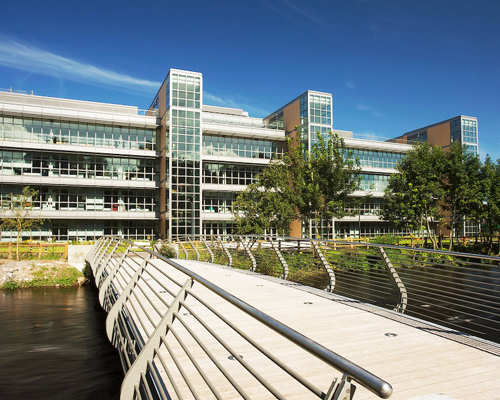
\includegraphics[width=3in]{img/WGB.jpg}
\caption{Western Gateway Building: home to CSIT}
\label{fig:wgb}
\end{SCfigure}


\newpage 
\subsection{Analyse three years of data on undergraduate students by}
\label{sec:ug_data}
\instr{
\begin{itemize}
\item gender and degree programme, with reference to discipline-specific benchmark data; 
\item gender and degree attainment;
\item gender and foundation courses.  
\end{itemize}
}

\subsubsection{Three years of data on undergraduate students by gender and degree programme}

Figure~\ref{fig:ug:enrolment} summarises enrolment statistics for our
undergraduate  programmes for  2017-18 to 2019-20 by gender.\footnote{BScDSA and BAPC started  in 2018-19.} 
The gender balance is markedly better for the interdisciplinary 
programmes, especially the two BA programmes.  


\begin{figbox}
    \caption{Enrolment undergraduate students 2017-2020}
    \label{fig:ug:enrolment}
    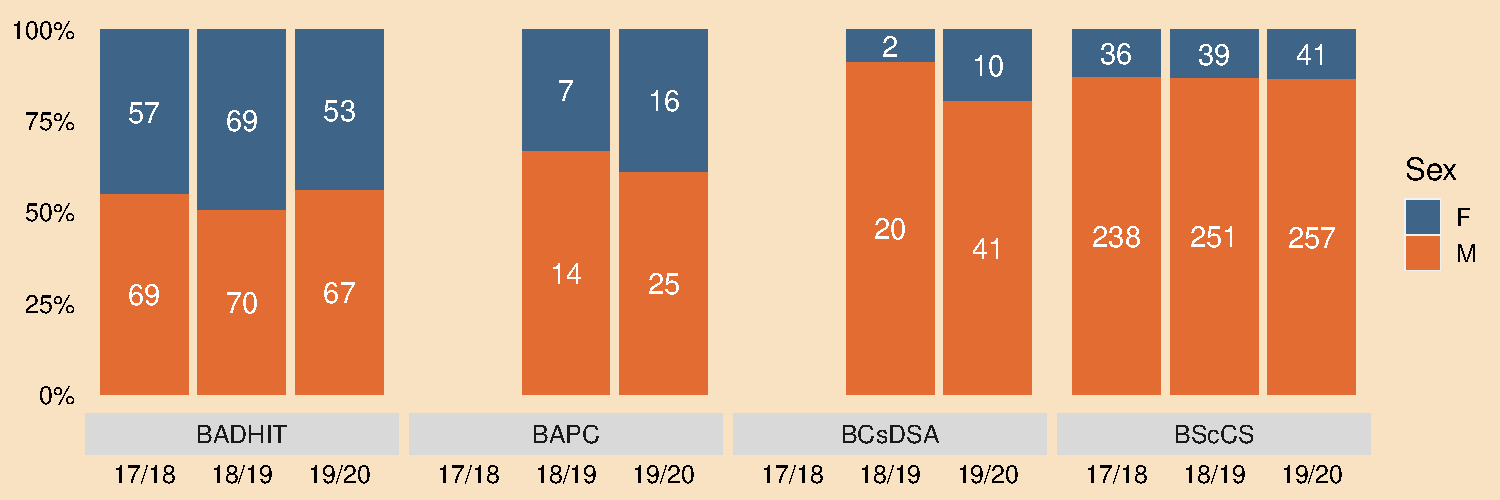
\includegraphics[width=\textwidth]{fig/ug_enrolment2.pdf}
\end{figbox}

From Figure~\ref{fig:ug:enrolment} 
our undergraduate programmes exhibit wide variation in
female enrolment rates from 14-16\% in the BScCS
to 44-50\% in BADHIT. As the  former aligns better
with the school's research programmes, any increase in female 
undergraduate numbers there will provide a bigger pool 
of potential research postgraduates over time.

Figure~\ref{fig:ug:mfintake} shows the evolution of the gender
breakdown linked to the introduction of new programmes
(BScDSA, BADHIT, BAPC), showing that these have improved 
the overall  gender balance  without adversely affecting 
the female participation rate for the established BScCS.
In 2009-10, prior to the introduction of these newer 
programmes, the percentage of females was 14\%, compared 
with $24-25\%$ for the period shown.


\begin{figbox}
    \caption{Evolution of male/female intake for the BSc. CS programme vs. other undergraduate programmes within CSIT}
    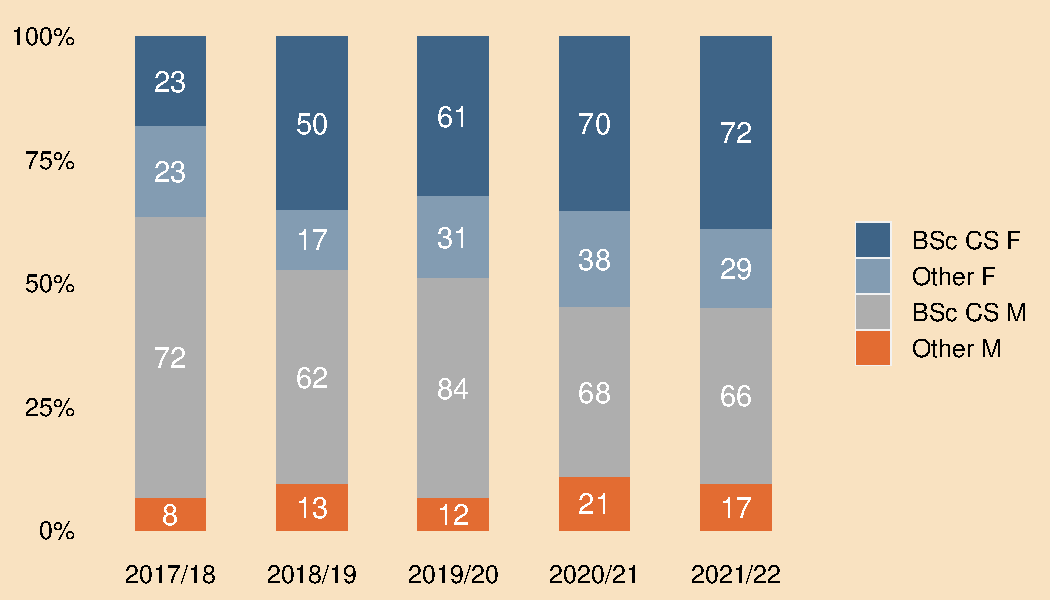
\includegraphics[width=5in]{fig/mfintake.pdf}
    \label{fig:ug:mfintake}
\end{figbox}

Table~\ref{tab:benchmarking:ug} compares CSIT's gender participation
rates for undergraduate  programmes with Irish (HEA) and UK (HESA)
bemchmarks. CSIT's 22-24\% is somewhat better than the Irish (HEA) 
figure of 19-20\% and 15-16\% for the UK (HESA). 

% KH: Modified 25 October 22 to strip out raw
% numbers leaving just percentages.


\begin{tabbox}{!th}


\caption{Percentage of females on undergraduate 
programmes  for full-time students, benchmarked 
nationally (HEA) and with the 
UK (HESA)}
\label{tab:benchmarking:ug}
\footnotesize       
\sisetup{
    group-digits=all,
    group-separator = {,},
    group-minimum-digits=4,
    table-format=5.0,
    reset-text-series = false, 
    text-series-to-math = true
}
\begin{tabular}{p{2cm} 
                %S[table-format=3.1]
                %S[table-format=3.1]
                S[table-format=3.0\%]
                p{0.7cm}
                %S[table-format=3.0]
                %S[table-format=5.0]
                S[table-format=3.0\%]
                p{0.7cm}
                %S[table-format=6.0]
                %S[table-format=6.0]
                S[table-format=3.0\%]}
\toprule
Year
  & \textmd{UCC CSIT} 
  &
  &\textmd{HEA\textsuperscript{1}}
  &
  &\textmd{HESA\textsuperscript{2}}\\
%  \cmidrule{2-4}\cmidrule{6-8}\cmidrule{10-12}
 \midrule 
2017-18 &22\% && 19\% &&15\%\\
\hdashline
2018-19 &25\% &&19\% &&15\%\\
\hdashline
2019-20 &24\% &&20\% &&16\%\\ 
%   & \multicolumn{3}{c}{\textbf{UCC CSIT}} 
%   &
%   &\multicolumn{3}{c}{\textbf{HEA (Ireland)}} 
%   &
%   &\multicolumn{3}{c}{\textbf{HESA (UK)}}\\
%   \cmidrule{2-4}\cmidrule{6-8}\cmidrule{10-12}
% Year & {F}& {M} & {F\%} & & {F}& {M}& {F\%} & & {F} & {M} & {F\%}\\ 
%  \midrule 
% 2017-18 & 95  & 344 & 22\% && 908 & 3762 & 19\% && 11080 &63250 &15\%\\
% 2018-19 & 117 & 355 & 25\% && 871 & 3664 & 19\% && 11965 &65935 &15\%\\
% 2019-20 & 121 & 390 & 24\% && 910 & 3755 & 20\% && 13635 &69800 &16\%\\ 
\bottomrule 
\end{tabular}
\vspace{2mm}\\
{
\sffamily

\textsuperscript{1}\ac{HEA} percentages reflect programmes classified as \ac{ICT} 
(\ac{ISCED});\\
\textsuperscript{2}\ac{HESA} reflect programmes under heading
of Computing. 

%     The \ac{HEA} used the \ac{ISCED} and reports students studying \ac{ICT}, which % covers ICT, Database and Network 
% Design, and Software and Applications Development and Analysis. From 2019/2020 % interdisciplinary programmes 
% incorporating ICT are also included.
%     The UK \ac{HESA} \ac{HeCoS} aggregates the following subjects as Computing; % computer science, information 
%technology, information systems, software engineering, artificial intelligence, 
% computer games and animation, 
% business computing, and others in computing.

}


\end{tabbox}


\subsubsection{Three years of data on undergraduate students by gender and 
degree attainment}


Figure~\ref{fig:ug:attainment} summarises the degree classifications received  
by graduating students for the BScCS and the BADHIT. (The first graduates for 
the other two UG programmes emerged only in 2021-22.)
Females are well represented among those  receiving higher degree classifications 
in both programmes. For the BScCS, no clear gender pattern is evident regarding 
higher grades (2H1 and 1H), however no females received the lower grades 
(Pass, 3H). For the BADHIT, the proportion of females receiving higher grades 
(2H1, 1H) was higher than for their male classmates for two of the three
years shown.

\begin{figbox}
    \caption{Degree attainment BScCS}
    \label{fig:ug:attainment}
    %\includegraphics[width=\textwidth]{fig/bsc_attainment2
    \begin{subfigure}[t]{2.9in}
    \caption{Degree attainment BScCS}
    \label{fig:bsc:attainment}
    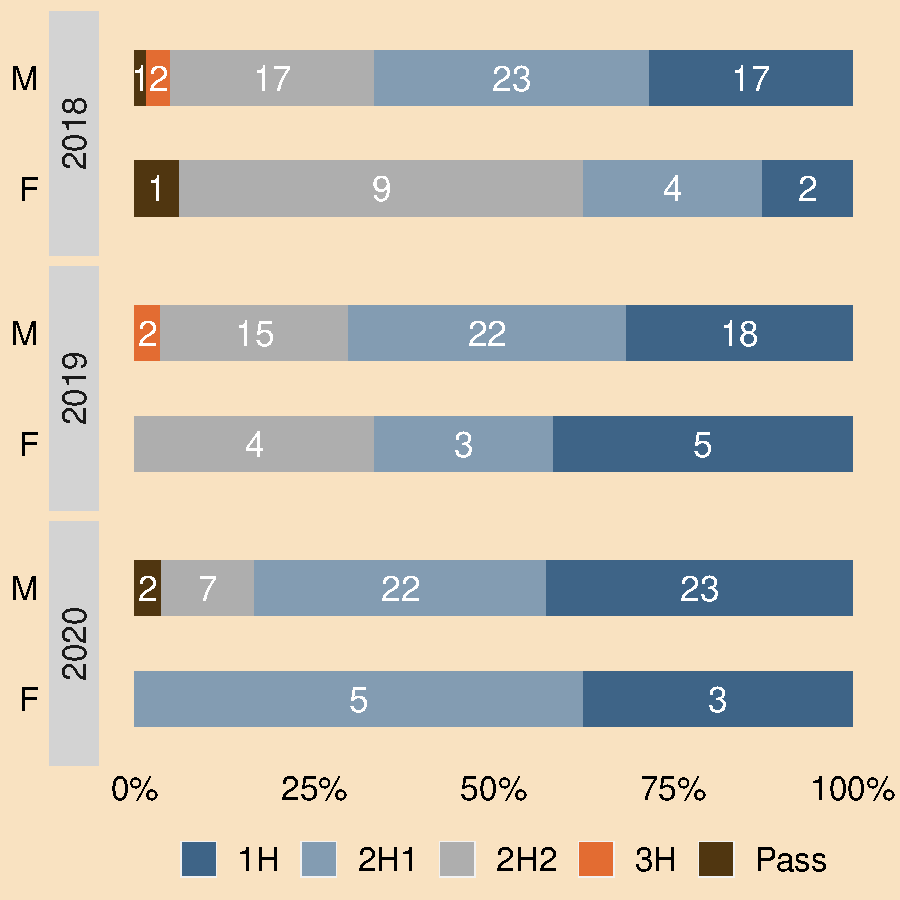
\includegraphics[width=2.8in]{fig/ug_attain2.pdf} % NEW
    \end{subfigure}
    %\includegraphics[width=4in]{fig/bsc_attainment2.pdf} %% OLD
    %
    \begin{subfigure}[t]{2.8in}
    \caption{Degree attainment BADHIT}
    \label{fig:badhit:attainment}
    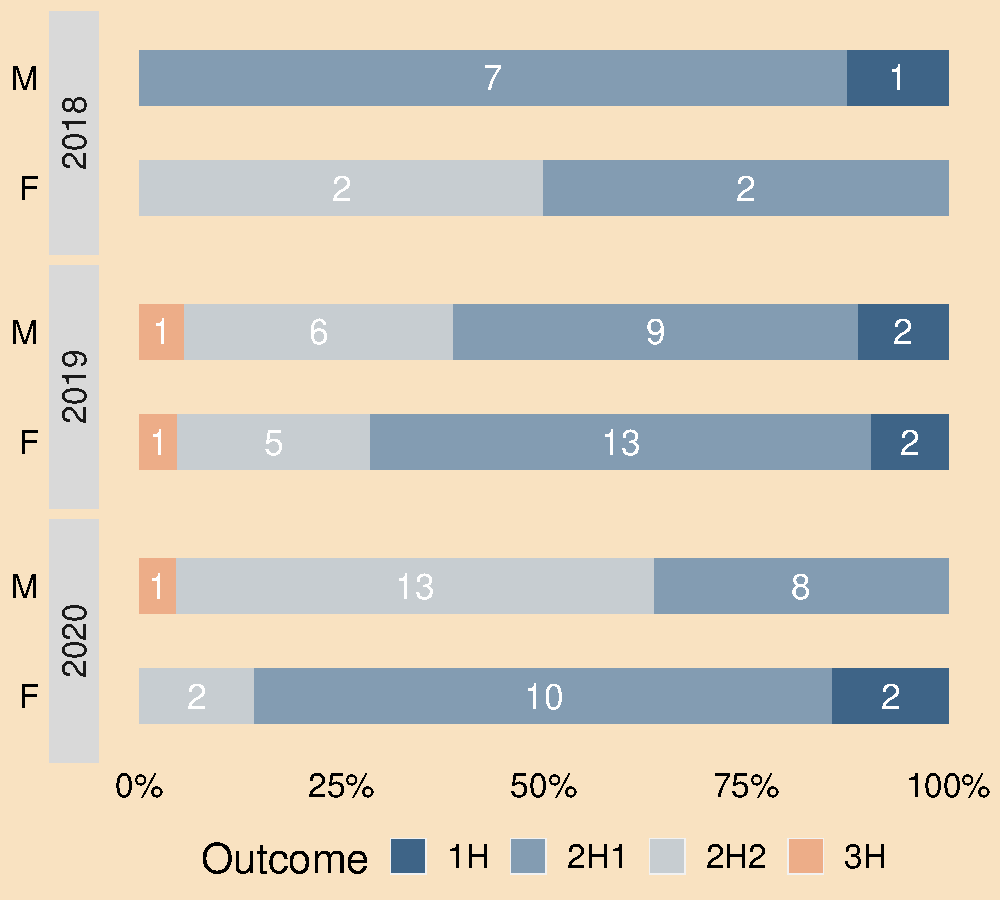
\includegraphics[width=2.8in]{fig/badhit_attainment2.pdf}
    \end{subfigure}
    
\end{figbox}



\begin{figbox}

 \caption{Degree attainment undergraduate students across all 4 undergraduate programmes (2022)}
    %\centering
    \begin{subfigure}{2.8in}
    \caption{BSc CS}
    \label{fig:hdip}
    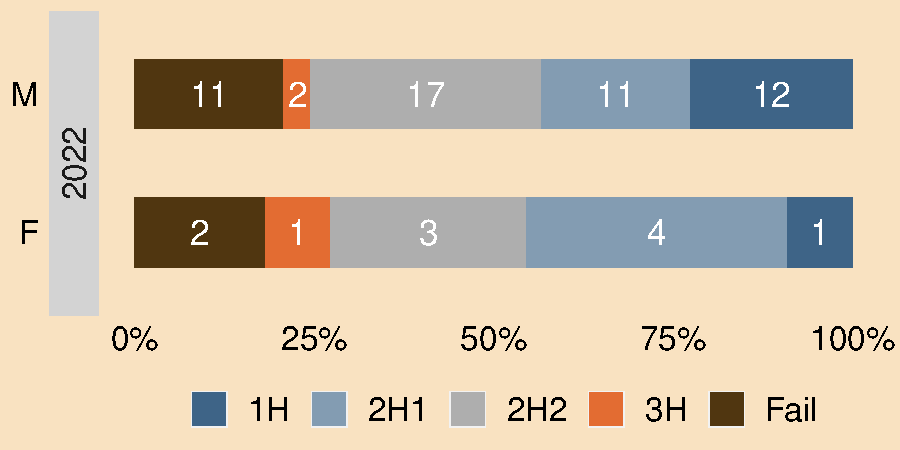
\includegraphics[width=2.8in]{fig/ug_attain_bsc22.pdf}
    \end{subfigure}
    %
    \begin{subfigure}{2.8in}
    \caption{BADHIT}
    \label{fig:msccs}
    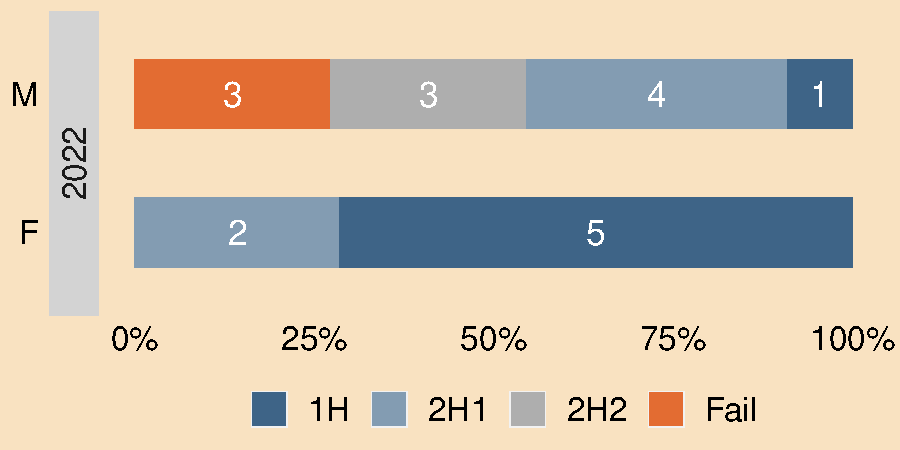
\includegraphics[width=2.8in]{fig/ug_attain_badhit22.pdf} 
    \end{subfigure}
    %
    \par\bigskip
    %
    \begin{subfigure}{2.8in}
    \caption{BAPC}
    \label{fig:mscdsa}
    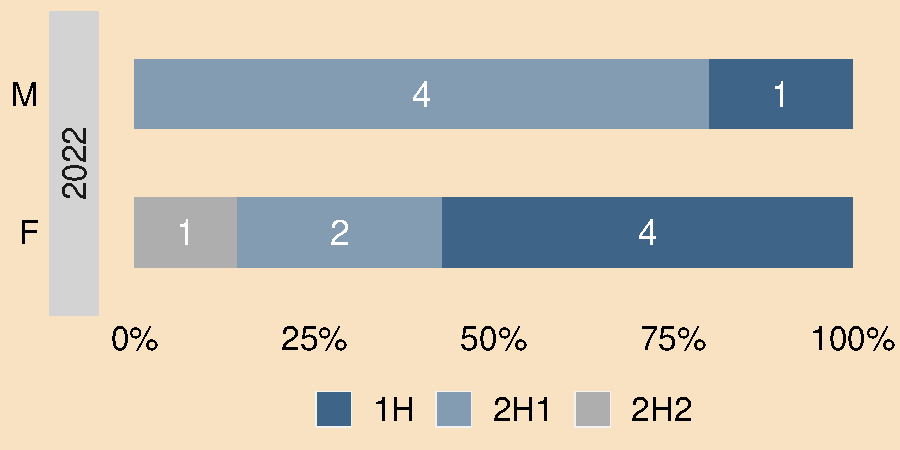
\includegraphics[width=2.7in]{fig/ug_attain_bapc22.pdf} 
    \end{subfigure}
    %
    \begin{subfigure}{2.8in}
    \caption{BSc DSA}
    \label{fig:mscim}
    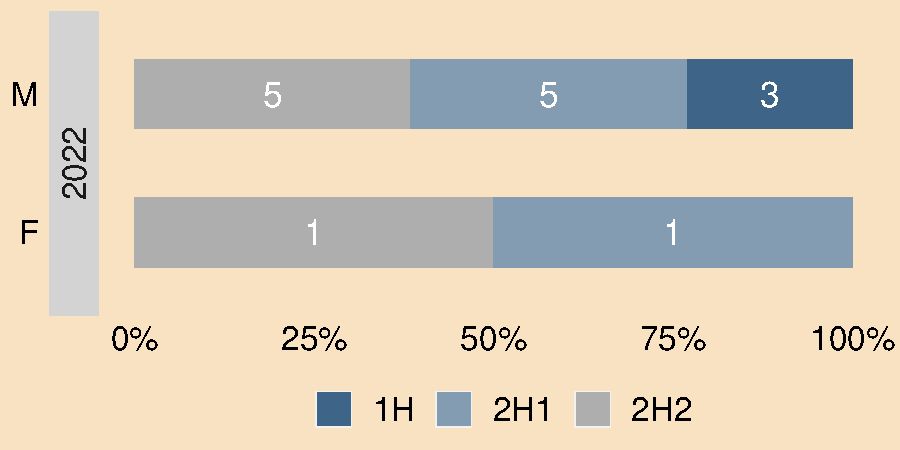
\includegraphics[width=2.7in]{fig/ug_attain_bscdsa22.pdf} 
    \end{subfigure}
    %
    \par 
    %% Add the legend
   
    % \begin{subfigure}{14cm}
    % \centering 
    % % left bottom right top
    % 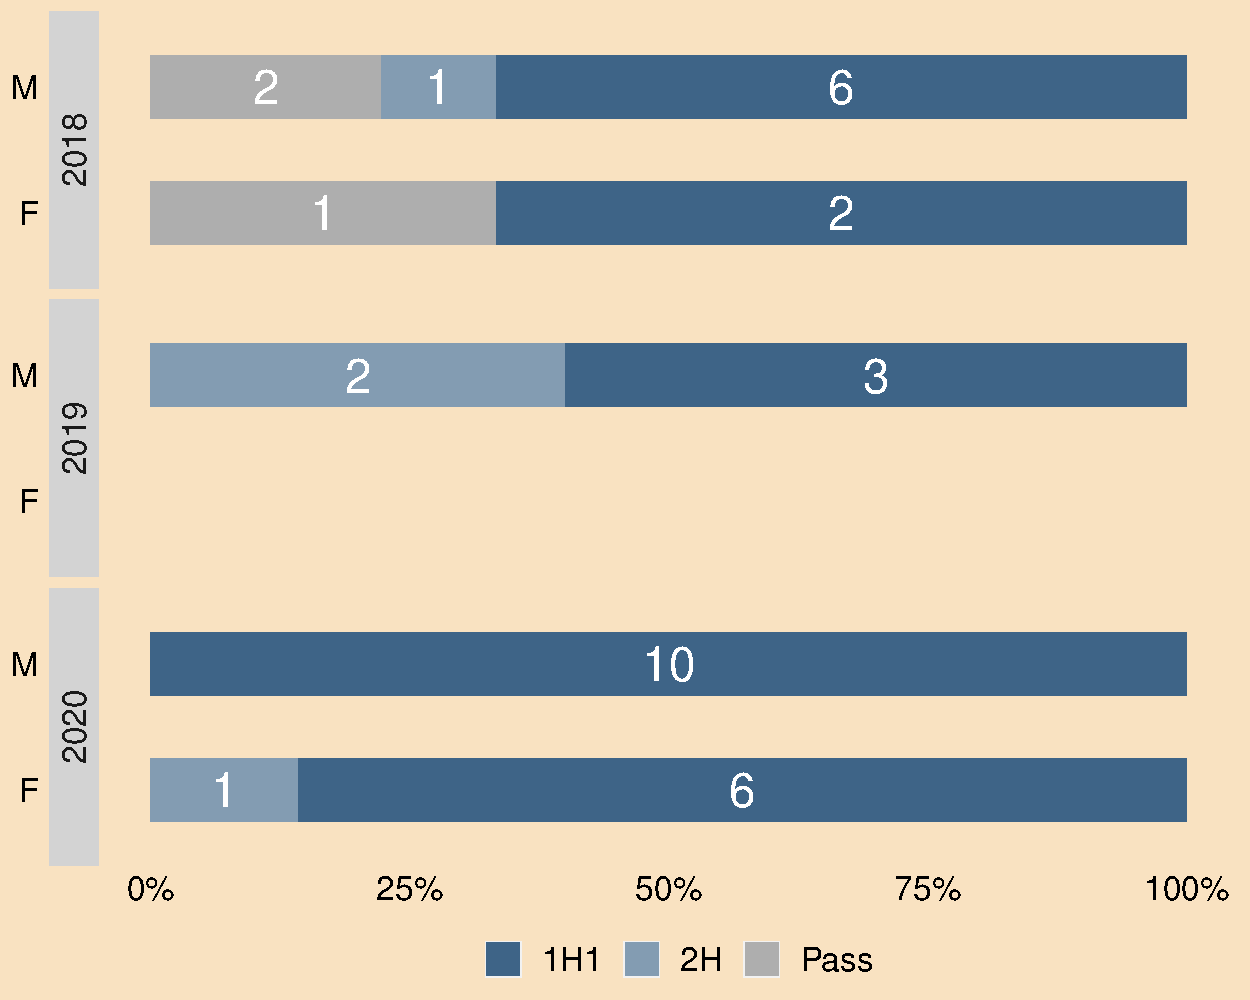
\includegraphics[trim={0 0 0 15.5cm},clip,width=3in]{fig/pg_legend.pdf} 
    % \end{subfigure}
    
    \label{fig:ug:attainment:all}

\end{figbox}


\subsubsection{Data on undergraduate students by gender and foundation courses}

No foundations courses offered.


\subsection{Analyse three years of data on postgraduate taught students by:} 
\instr{
\begin{itemize}
    \item gender and degree programme, with reference to discipline-specific benchmark data;  
    \item gender and degree attainment.  
\end{itemize}
}
\label{pg_data}


\subsubsection{Three years of data on postgraduate students by gender and degree 
programme}


Figure~\ref{fig:pg:enrolment} shows enrolment  for our taught
postgraduate programs for 2017-18 to 2019-20. Generally the female 
participation rate is significantly better for postgraduate
programmes than for undergraduate. The MScIM, which draws students 
with non-computing backgrounds, is the only programme
where females (56-68\%)  outnumber males. Both MScCS and MScDSA 
have a high proportion of non-EU students and a significantly 
better gender balance is evident, possibly due higher participation 
among females in STEM subjects in some non-EU cultures.


\begin{figbox}
    \caption{Enrolment postgraduate students 2017-2020}
    \label{fig:pg:enrolment}
    %\centering
    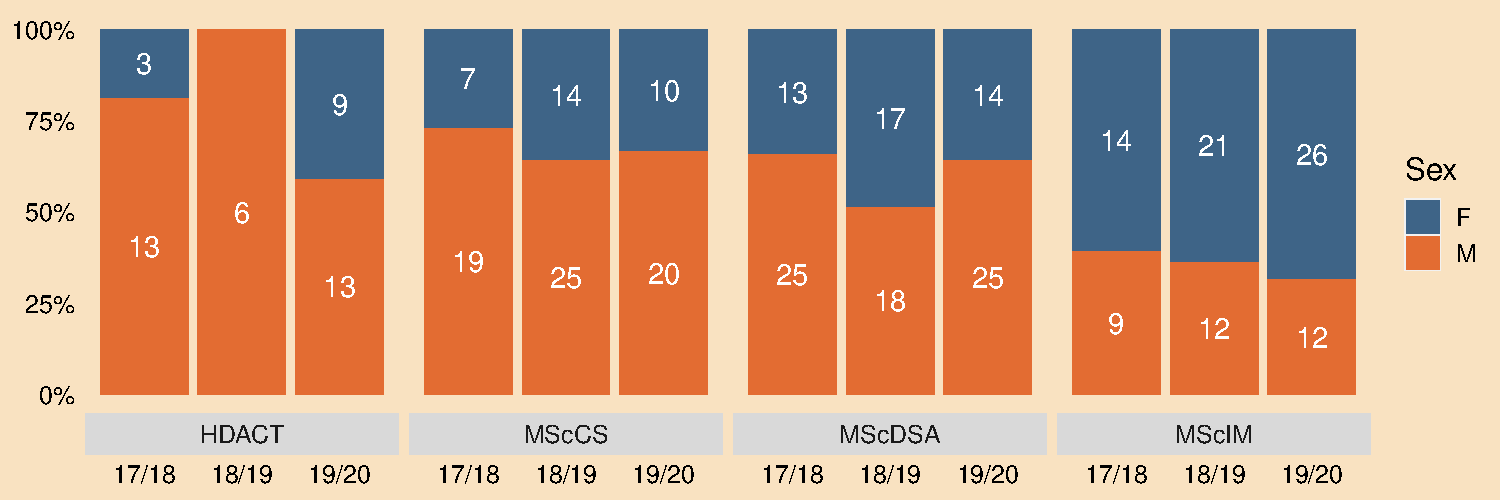
\includegraphics[width=\textwidth]{fig/pg_enrolment.pdf}
\end{figbox}


% KH: modified 25 Oct 22 to strip out raw numbers
% and leave percentages. This declutres and also 
% disguises some discrepancies.

\begin{tabbox}{!th}
      
\footnotesize       
\caption[Percentage of females on postgraduate taught programmes, benchmarked nationally
(HEA) and with the UK (HESA)]{Percentage of females on postgraduate taught programmes, benchmarked nationally
(HEA) and with the UK (HESA) (full-time students only)}
\label{tab:benchmarking:pg}

\sisetup{
    group-digits=all,
    group-minimum-digits=4,
    group-separator = {,},
    table-format=4.1,
    mode=text,
    reset-text-series = false, 
    text-series-to-math = true,
    reset-text-family = false, 
    text-family-to-math = true
}
\begin{tabular}{p{2cm} 
                %S[table-format=3.1]
                %S[table-format=3.1]
                S[table-format=3.0\%]
                p{0.7cm}
                %S[table-format=3.1]
                %S[table-format=3.1]
                S[table-format=3.0\%]
                p{0.7cm}
                %S[table-format=4.1]
                %S[table-format=5.1]
                S[table-format=3.0\%]}
\toprule
  Year
  & \textmd{UCC CSIT}
  &
  &\textmd{HEA} 
  &
  &\textmd{HESA}\\
%  \cmidrule{2-4}\cmidrule{6-8}\cmidrule{10-12}
%Year & {F}& {M} & {F\%} & & {F}& {M}& {F\%} & & {F} & {M} & {F\%}\\ 
\midrule 
2017-18 &37\% &&29\%  &&30\%\\
\hdashline
2018-19 &45\% &&32\% &&31\%\\
\hdashline
2019-20 &43\% &&32\% &&30\%\\
\bottomrule 
\end{tabular}

\end{tabbox}



From Figure~\ref{fig:pg:enrolment} shows an improvement of
female participation rates over the period presented from 
37\% to 43\% and as Table~\ref{tab:benchmarking:pg} shows  
CSIT's rate of 37-45\% is significantly that the HEA, HESA 
figures of 29-32\% and 30-31\% respectively.

\subsubsection{Three years of data on postgraduate students by gender 
and degree attainment}

Figure~\ref{fig:pg:attainment} plots the degree classifications
achieved for those completing the four taught postgraduate 
programmes over the period 2017-18 to 2019-29. No obvious
gender pattern is apparent, though as with the undergraduate
programmes, females feature prominently among those receiving 
higher grades.

\begin{figbox}

 \caption{Degree attainment postgraduate students}
    %\centering
    \begin{subfigure}{2.8in}
    \caption{Postgraduate attainment HDip ACT}
    \label{fig:hdip}
    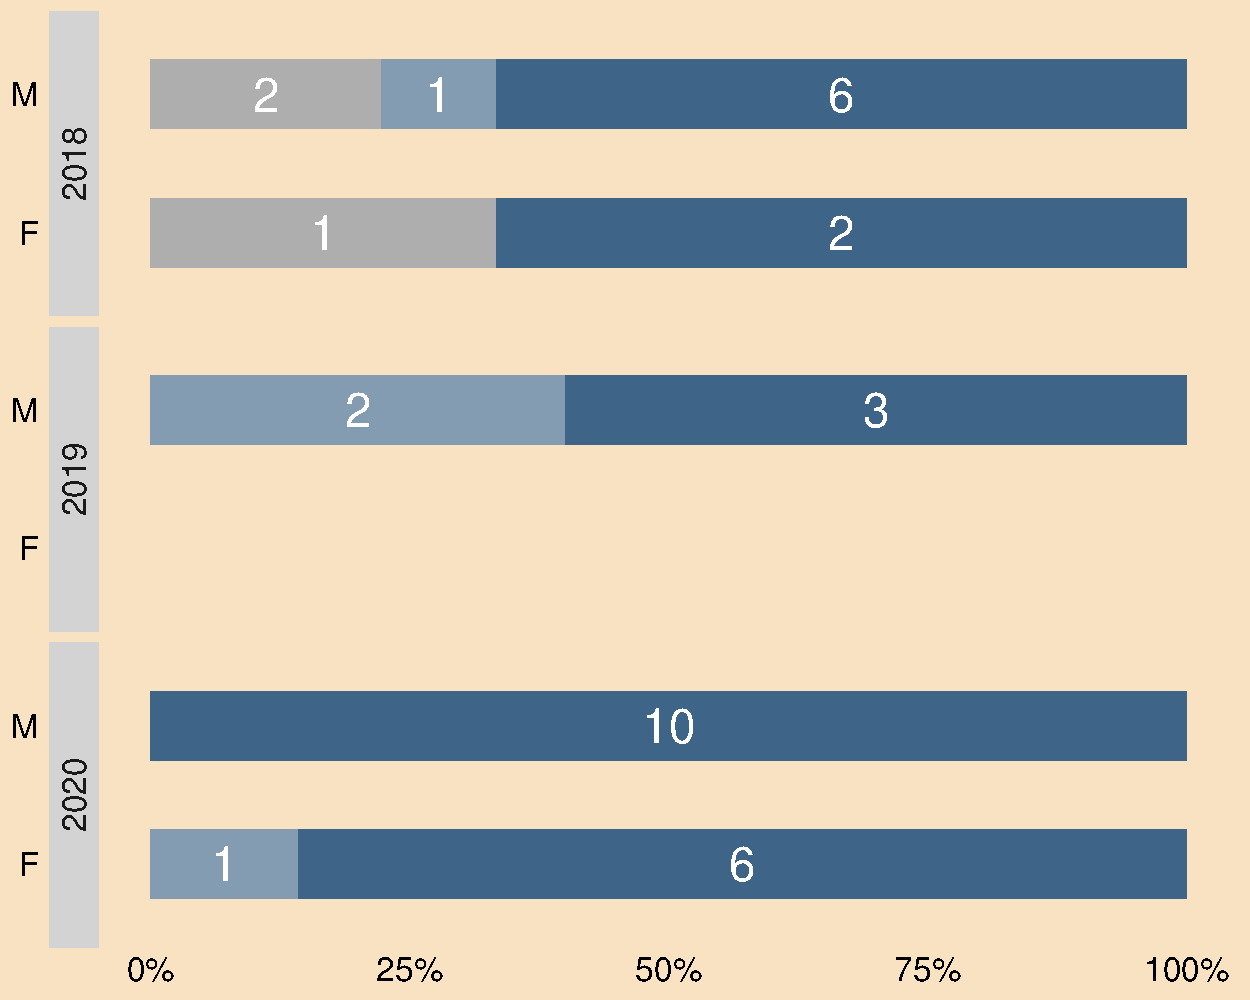
\includegraphics[width=2.8in]{fig/pg_hdact_attainment.pdf}
    \end{subfigure}
    %
    \begin{subfigure}{2.8in}
    \caption{Postgraduate attainment MSc CS}
    \label{fig:msccs}
    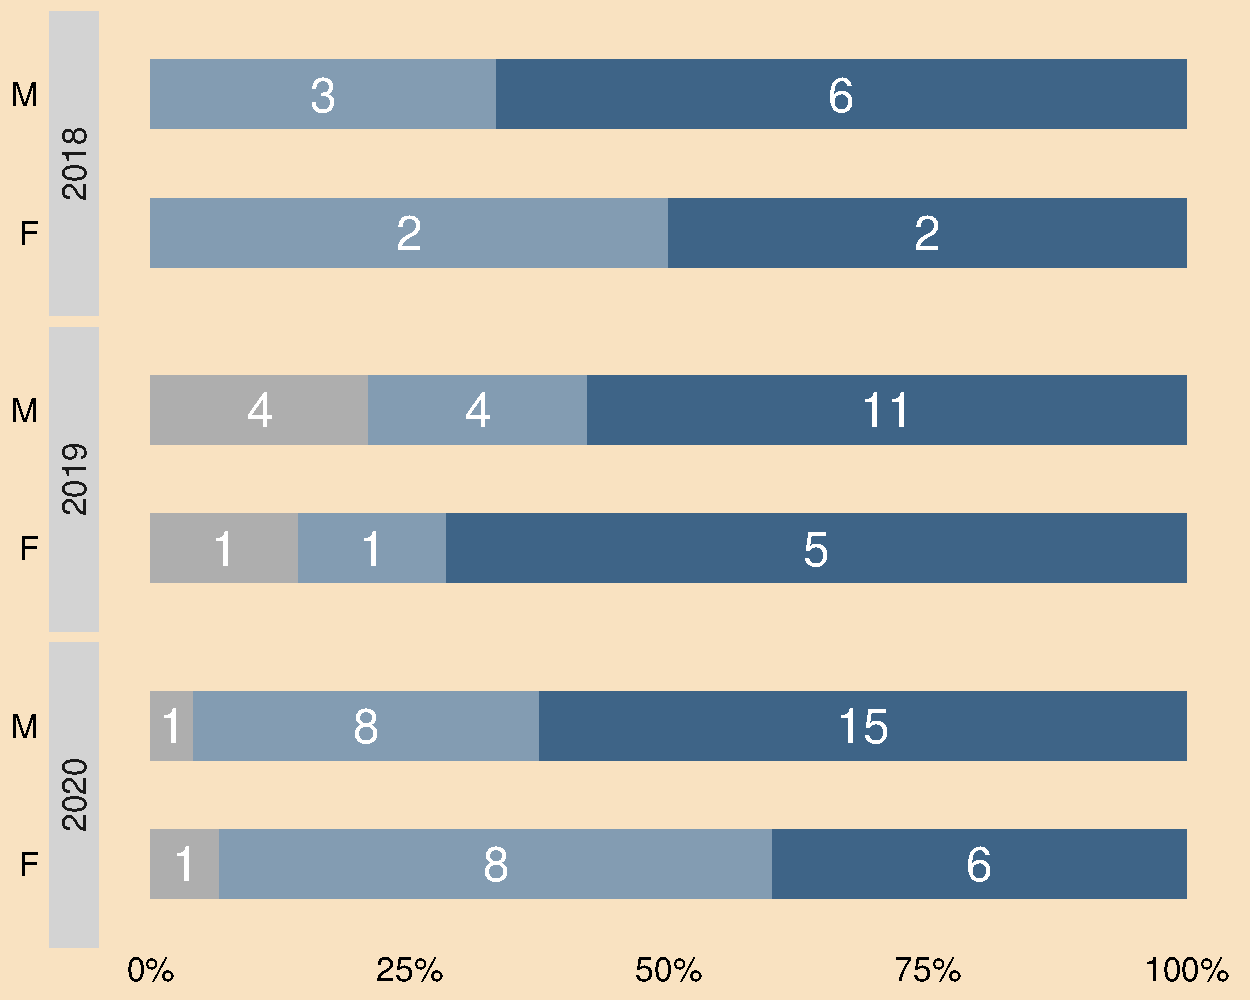
\includegraphics[width=2.8in]{fig/pg_msccs_attainment.pdf} 
    \end{subfigure}
    %
    \par\bigskip
    %
    \begin{subfigure}{2.8in}
    \caption{Postgraduate attainment MSc DSA}
    \label{fig:mscdsa}
    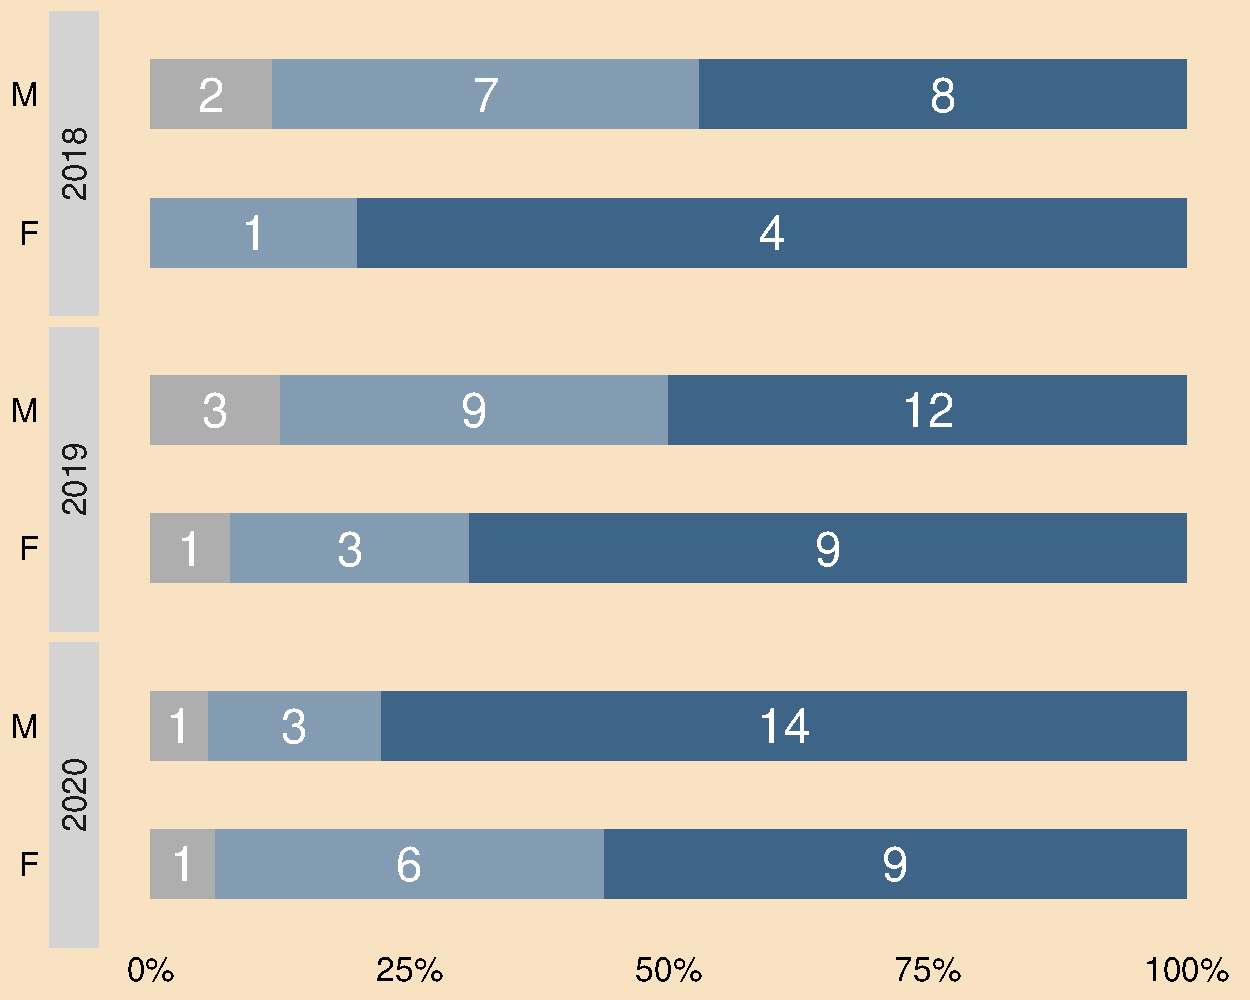
\includegraphics[width=2.7in]{fig/pg_mscdsa_attainment.pdf} 
    \end{subfigure}
    %
    \begin{subfigure}{2.8in}
    \caption{Postgraduate attainment MSc IM}
    \label{fig:mscim}
    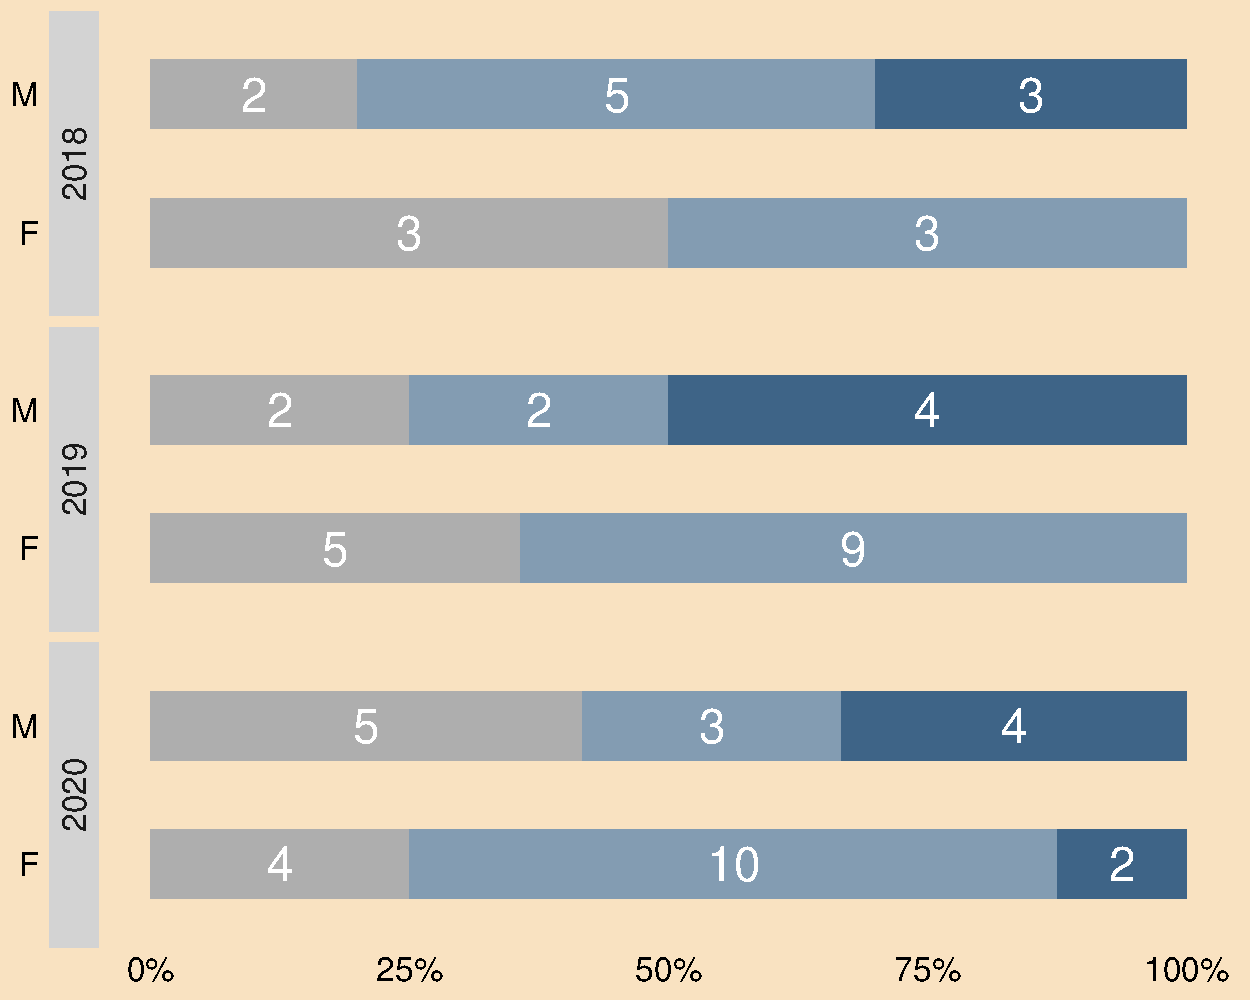
\includegraphics[width=2.7in]{fig/pg_mscim_attainment.pdf} 
    \end{subfigure}
    %
    \par 
    %% Add the legend
   
    \begin{subfigure}{14cm}
    \centering 
    % left bottom right top
    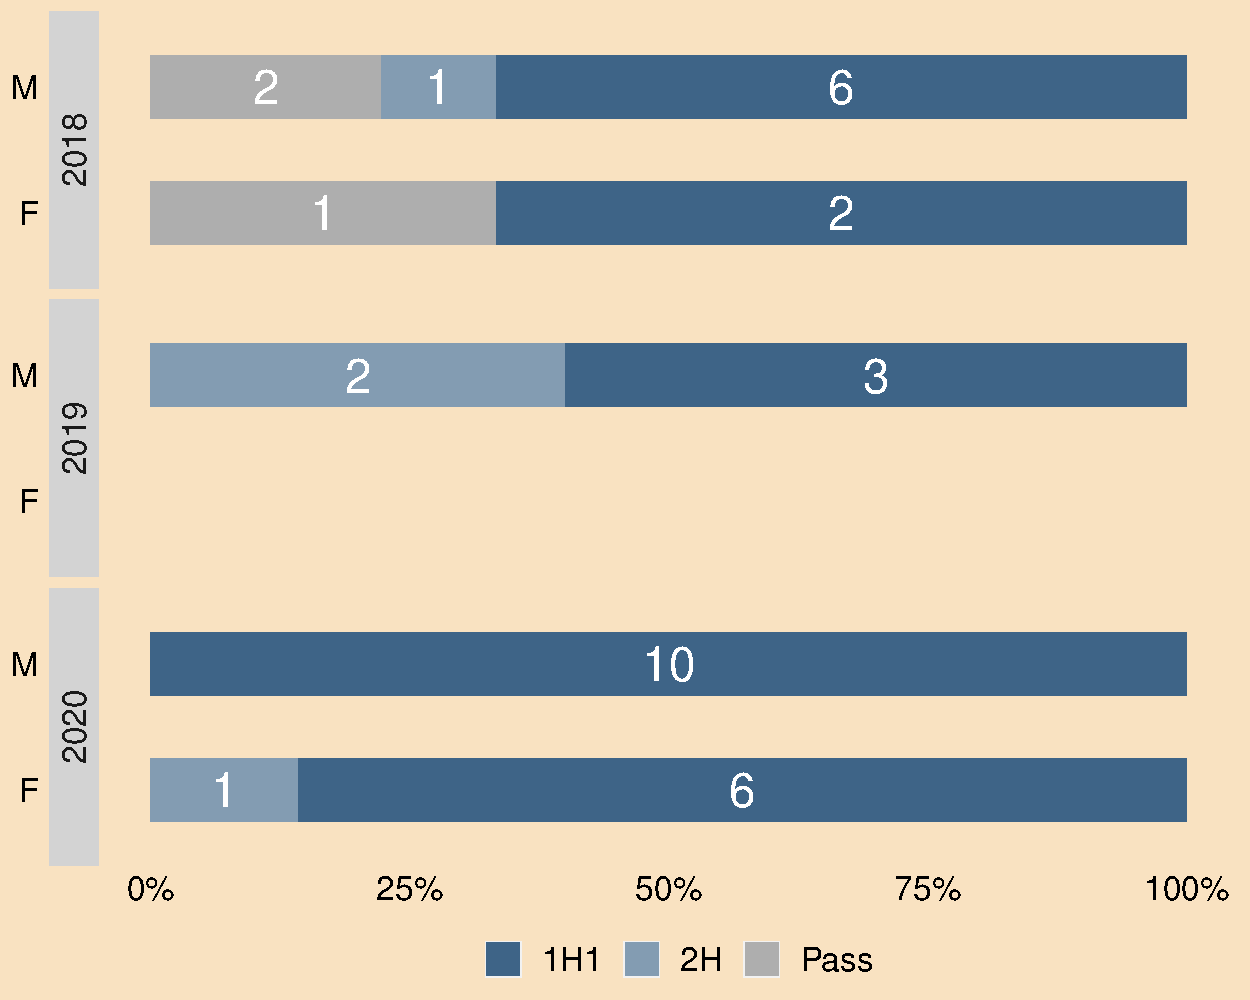
\includegraphics[trim={0 0 0 15.5cm},clip,width=3in]{fig/pg_legend.pdf} 
    \end{subfigure}
    
    \label{fig:pg:attainment}

\end{figbox}


\subsection{Analyse three years of data on postgraduate research 
students by:}  
\instr{
\begin{itemize}
    \item gender and enrolment; 
    \item gender and application, offer, and enrolment, with comment on how this data is collected and evaluated by the department, and on any gender disparities in student funding;  
    \item gender and completion rates.  
\end{itemize}
}
\label{sec:phdstudents}


\subsubsection{Three years of data on postgraduate research students 
by gender and enrolment}
\label{sub:phdnumbers}


Table~\ref{tab:phdregistrations} shows the number of
PhD students registered for  2017-18 to 2019-20. 

% \begin{figure}[!ht]
%     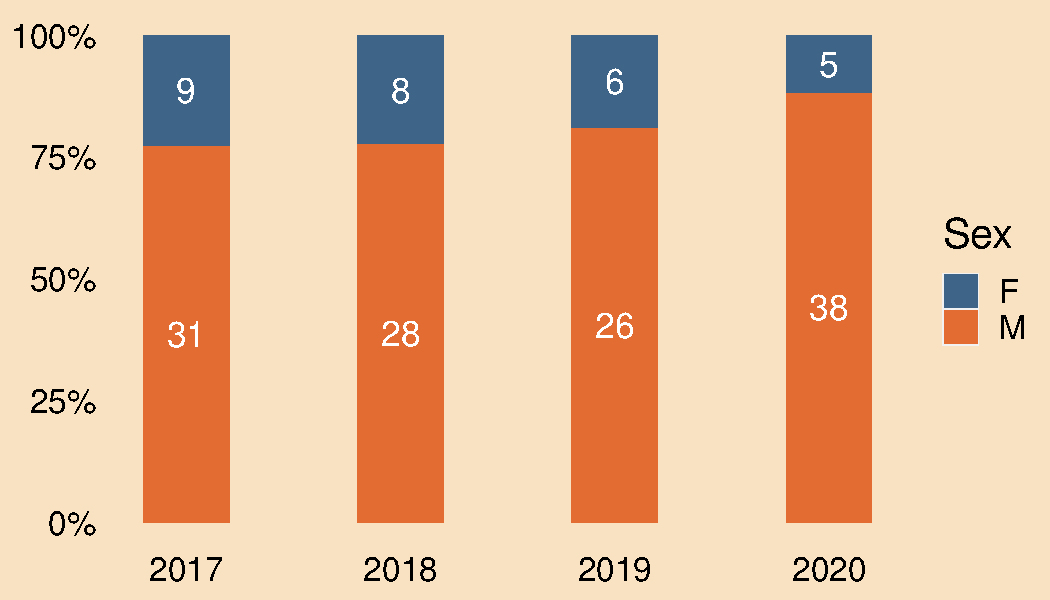
\includegraphics[width=3in]{fig/phd_registered.pdf}
%     \caption{Total enrolment numbers of PhD students (2017-2020)}
%     \label{fig:phdenrolments}
% \end{figure}

% Data for 2017-18 to 2019-20 taken from EDI spreadsheet
% Sheet K.
%
%

\begin{tabbox}{!th}
\caption{Number of PhD students registered from 2017-18 to 2019-20 by  gender}
\label{tab:phdregistrations}
\footnotesize 

\sisetup{
    group-digits=all,
    group-minimum-digits=4,
    mode=text,
    reset-text-series = false, 
    text-series-to-math = true,
    reset-text-family=false, 
    text-family-to-math=true
}


\begin{tabular}{p{3cm}
                R{1cm}
                C{1.2cm}           
                C{1.3cm}
                R{1cm}
                }
\toprule                 
\textmd{Year}&
\textmd{M}&
\textmd{F}&
\textmd{Total}&
\textmd{\%F}\\ 
\midrule 
2017-18&30 &11 &41 & 33\%\\
\hdashline
2018-19&26 &19 &45 & 28\%\\
\hdashline
2019-20&39 &6 &45 & 13\%\\
\bottomrule 
\end{tabular}


\end{tabbox}




The dip in 2019-20 reflects the ending of one funding source,
before the start of the two Centres for Research Training (CRT)
in 2019. These CRTs have explicit targets for 
increased female PhD students (40\%), which has driven an 
increase in the intake of female PhD students, as shown in Table~\ref{tab:phdintakerecent}.
As SFI has gender targets attached to other funding, a similar 
pattern is expected among the non-CRT PhD intake in future years.


\begin{tabbox}[5.8cm]{!th}
\caption{CSIT PhD Registrations since 2019-20}
\label{tab:phdintakerecent}
\footnotesize 

\sisetup{
    group-digits=all,
    group-minimum-digits=4,
    table-format=2.1,
    mode=text,
    reset-text-series = false, 
    text-series-to-math = true,
    reset-text-family=false, 
    text-family-to-math=true
}

% \begin{tabular}{cccccc}
% \multicolumn{2}{c}{2019-20} &
% \multicolumn{2}{c}{2020-21} &
% \multicolumn{2}{c}{2021-22} \\
% M & F & M & F & M & F\\
% 15 & 4 & 13 & 9 & 5 & 6\\
% & 21\% & & 41\% & & 55\%\\
% \end{tabular}

\begin{tabular}{p{3cm}
                S[table-format=2.0]
                !{\qquad}
                S[table-format=2.0]
                !{\qquad}
                S[table-format=2.0\%]}
\toprule
Year & {M} & {F} & {\%F} \\
\midrule
2019/2020 & 15 & 4 & 21\%\\
\hdashline
2020/2021 & 13 & 9 & 41\%\\
\hdashline
2021/2022 &  5 & 6 & 55\%\\
\bottomrule 
\end{tabular}


\end{tabbox}


The intake by research centre or CRT for 2022-23 is shown in 
Table~\ref{tab:phdregistrations2223}.


\begin{tabbox}{!th}
\caption{CSIT PhD students registered 2022-23
by centre and gender}
\label{tab:phdregistrations2223}
\footnotesize 

\sisetup{
    group-digits=all,
    group-minimum-digits=4,
    mode=text,
    reset-text-series = false, 
    text-series-to-math = true,
    reset-text-family=false, 
    text-family-to-math=true
}


\begin{tabular}{p{3cm}
                R{1cm}
                R{1cm}           
                R{1cm}
                R{1cm}
                }
\toprule                 
\textmd{Research Centre}&
\textmd{M}&
\textmd{F}&
\textmd{Total}&
\textmd{\%F}\\ 
\midrule 
Advance-CRT&
12& 8& 20& 40\%\\
\hdashline
CRT-AI&
8& 4& 12& 33\%\\
\hdashline
Insight&
11& 5& 14& 36\%\\
\hdashline
Other&
11& 4& 15& 27\%\\
\midrule 

Total&
42& 21& 63& 33\%\\

\bottomrule 
\end{tabular}
\vspace{2mm}\\
{
\sffamily

Other includes students attached to research centres such as 
MISL, Confirm, Lero and Enable.
}

\end{tabbox}




PhD students are funded in full either through their CRT or research 
centre or supervisor for the four years of their PhD studies. The 
funding profile by gender mirrors the enrolment profile.

\subsubsection{Three years of data on postgraduate research students by gender, 
application, offer, and enrolment}
\label{sec:phdnumbers}

% \akcomment{Section 2.1.d - 1. data on application, offer, enrolment incomplete; 
% application questions on how this data is collected and evaluated by the School 
% need to be addressed; also the question seeking comment on gender disparities on 
% student funding needs to be addressed. 2. PGR completion rates - comment is 
% needed on gender differences in completion rates (if any). Completion rates are 
% calculated based on corresponding intake data - do you have this?  Only on-time 
% completion data is provided here, but it's difficult to contextualise without 
% access to completion rates.
% }


Historically, the PhD application process was handled by individual 
centres or PIs and while centres maintained records locally, no records 
were maintained at school level to monitor the overall gender breakdown 
of the number of applicants, offers and acceptances. Indeed, gender 
information was often not requested of applicants. 
Action~\ref{PHDMETRICS} will address this.


Table~\ref{tab:crtapplications} summarises the
number of applications and enrolments by gender for the two CRTs
since their introduction in 2019. CRTs are national
consortia and the application process is handled at consortium 
level and students matched with specific institutions and supervisors 
subsequently. Hence, it is not possible to dis-aggregate applications 
by institution.

\begin{tabbox}{!h}

\caption{CRT data on applications and enrolments by gender}
\label{tab:crtapplications}
\footnotesize 

\sisetup{
    group-digits=all,
    group-minimum-digits=4,
    mode=text,
    reset-text-series = false, 
    text-series-to-math = true,
    reset-text-family=false, 
    text-family-to-math=true
}
\begin{tabular}{p{3.3cm}
                p{2cm}
                C{1cm}C{1cm}C{1cm}
                C{1cm}C{1cm}C{1cm}
                C{1cm}C{1cm}C{1cm}
               }
\toprule 
&& \multicolumn{6}{c}{National} & \multicolumn{3}{c}{UCC}\\
\cmidrule(l){3-8}\cmidrule(l){9-11}
& & \multicolumn{3}{c}{Applications} 
    &\multicolumn{3}{c}{Enrolments} &\multicolumn{3}{c}{Enrolments}\\
    \cmidrule(l){3-5}\cmidrule(l){6-8}\cmidrule(l){9-11}
Centre & Year & M & F & F\% & M & F & F\% & M & F & F\% \\
\midrule


CRT-AI & 2019 &145 &89 &38\% &17 &14 &45\% &3 &1& 25\%\\
\cdashline{2-11}
& 2020 &245 &110 &31\% &15 &16 &50\% &3 &1& 25\%\\
\cdashline{2-11}
&2021 &175 &65 &27\% &14 &9 &39\% &2 &2& 50\%\\
\hdashline
ADVANCE-CRT & 2019 &162 &54 &25\% &15 &7 & 32\%& 3&2 & 40\%\\
\cdashline{2-11}
&2020 &390 &139 &26\% &9 &10 &53\% &6 &4 & 40\%\\
\cdashline{2-11}
&2021 &291 &135 &31\% &16 &13 &45\%&2 &2 & 50\%\\
\bottomrule
\end{tabular}
{\\[.1in]
\sffamily 
The application process for CRTs is handled at consortium level and students are matched with specific institutions and supervisors. Hence, it is not possible to disaggregate applications by institution.
}
\end{tabbox}


For both CRTs the percentage of successful females exceeded the 
percentage among the applicant pool and the quota in two of the 
three years per CRT.


\subsubsection{Three years of data on postgraduate research students by gender 
and completion rates}

Figure~\ref{fig:phdcompletions} shows the number of PhD
completions for the period 2017-18 to 2019-20.

\begin{figbox}
    \caption{Number of PhD  completions (2017-2020)}
    \label{fig:phdcompletions}
    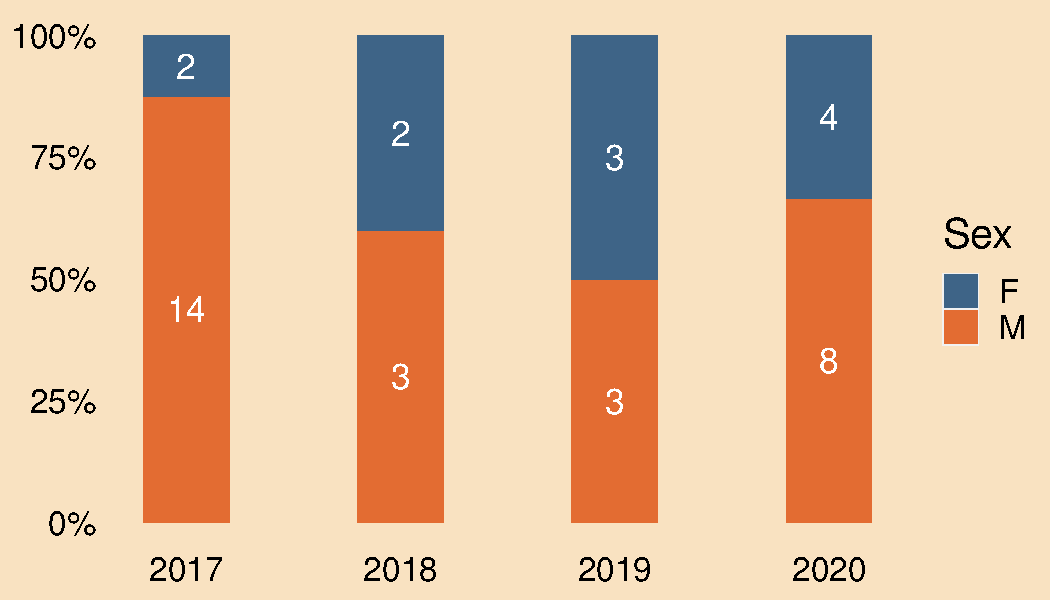
\includegraphics[width=3in]{fig/phd_completions.pdf}
\end{figbox}

Table~\ref{tab:phdcompletionrates} shows the completion rates 
for those who started from 2013-14 to 2015-16 (i.e. those expected
to finish during 2017-18 to 2019-20, assuming fours years to 
finish).

\begin{tabbox}{!th}
\caption{PhD completion rates by gender for those starting 2013-14 to 2015-16}
\label{tab:phdcompletionrates}
\footnotesize 

\sisetup{
    group-digits=all,
    group-minimum-digits=4,
    mode=text,
    reset-text-series = false, 
    text-series-to-math = true,
    reset-text-family=false, 
    text-family-to-math=true
}
\begin{tabular}{p{6cm}
                S[table-format=3.0]
                !{\quad}
                S[table-format=3.0]
                p{0.8cm}
                S[table-format=3.0]
                !{\quad}
                S[table-format=3.0]
                p{0.8cm}
                S[table-format=3.0]
                !{\quad}
                S[table-format=3.0]
                p{0.8cm}
                S[table-format=3.0]
                !{\quad}
                S[table-format=3.0]
               }
\toprule
& 
\multicolumn{2}{c}{2013-14}&&
\multicolumn{2}{c}{2014-15}&&
\multicolumn{2}{c}{2015-16}&&
\multicolumn{2}{c}{Total}\\
\cmidrule{2-3}\cmidrule{5-6}\cmidrule{8-9}\cmidrule{11-12}
& 
M & F && M & F && M & F && M & F\\
\midrule
Number new registrations&
6& 3&&
8& 2&&
10& 3&&
24& 8\\
\hdashline 
Number who completed&
5& 2&&
4& 2&&
7& 2&&
16& 6\\
\hdashline 
Average completion time (months)&
63& 71&&
59& 59&&
59& 60&&
60& 63\\
\hdashline 
Number yet to complete &
1& 0&&
1& 0&&
1& 0&&
3& 0\\

\bottomrule
\end{tabular}


\end{tabbox}


Table~\ref{tab:phdcompletiontimes} presents completion time data
by gender for those completing from 2017-18 to 2019-20, based
on registration and graduation data. As there may be a lag between 
``finishing up'' (viva voce, submission) and graduation, these 
figures may overstate the completion time somewhat.

\begin{tabbox}[9cm]{!th}

\caption{PhD time to graduation by gender for those completing during 2017-18 to 
2019-20}
\label{tab:phdcompletiontimes}
\sisetup{
    group-digits=all,
    group-minimum-digits=4,
    group-separator = {,},
    table-format=4.1,
    mode=text,
    reset-text-series = false, 
    text-series-to-math = true,
    reset-text-family = false, 
    text-family-to-math = true
}
\footnotesize   
\begin{tabular}{p{7cm} 
                S[table-format=2.0]
                !{\qquad}
                S[table-format=2.0]}
                

\toprule 
Duration & {M} & {F} \\
\midrule 
%4 years 
Up to 4 years, 5 months
& 4 & 0\\
\hdashline 
%5 years 
4 years, 6 months - 5 years, 4 months
& 12 & 4\\
\hdashline 
%6+ years 
5 years, 6 months and over
& 7 & 3\\

\bottomrule 
\end{tabular}
% {
% \sffamily 
% \\[.1in]
% * 4 years: up to 4 years and 5 months\\
% ** 5 years: 4.5 years to 5 years and 5 months\\
% *** 6+ years: 5.5 years and up\\
% }


\end{tabbox}


The completion time is marginally  worse for females (average 63 
months versus 60) as was the non-completion rate (25\% versus 20\%).  
Many students required more than four years to complete: three out 
of seven females took six years or more, compared to seven out of 
23 males. The numbers involved are too small on which to base firm 
conclusions, but it reinforce the need for school-level monitoring 
of PhD metrics to track these issues in future, as suggested in 
Action~\ref{PHDMETRICS}


\subsection{Comment and reflect on the relationship (if any) between the department’s outreach, engagement, and support activities and issues or opportunities in the student pipeline. This should include comment on how the department recognises staff and student contributions to these activities and monitors the gender balance of those involved.}


A benefit of the the self-assessment exercise is the realisation 
that we have never conducted a comprehensive audit of existing 
outreach, marketing and support activities to assess their 
effectiveness and reflect on how they might be reconfigured to 
mitigate the two key challenges in the student pipeline:
(1) the under-representation of females in certain undergraduate
programmes especially the BSc in Computer Science, and 
(2) the  small number of female undergraduates
who opt to progress to graduate research studies.


The school operates an Outreach Committee and participates in  a
range of outreach initiatives for prospective undergraduate 
students, including University events  (open days, careers 
guidance briefing sessions),  as well as hosting its own events 
such as an annual information evening, a popular programme of 
weekend programming activities and summer camps aimed at 
second-level students.

The School's outreach events are geared toward supporting gender 
diversity, and include secondary school visits and participation 
in the annual iWish event for women in science.
\footnote{\url{https://www.iwish.ie}} 
The School targets girls' schools in particular as shown in 
%Female staff are also invited to present at Schools, if interested. 
Table~\ref{tab:schoolvisits}. 
%In 2022, the Covid-19 pandemic had an impact on the schools visited. 
%Mixed schools saw the highest level of visits overall. 
While the School recognises the importance of visits to girls schools 
in particular, such school visits are dependent on the willingness 
of staff and the visited school to facilitate. 
%The table highlights there is an under-representation of girls schools visited.

\begin{tabbox}[10cm]{!th}

\caption{School visits to female-only, male-only, and mixed-gender schools}
\label{tab:schoolvisits}
\sisetup{
    group-digits=all,
    group-minimum-digits=4,
    group-separator = {,},
    table-format=4.1,
    mode=text,
    reset-text-series = false, 
    text-series-to-math = true,
    reset-text-family = false, 
    text-family-to-math = true
}
\footnotesize   
\begin{tabular}{p{3cm} 
                !{\qquad}
                S[table-format=2.0]
                !{\qquad}
                S[table-format=2.0]
                !{\qquad}
                S[table-format=2.0]
                !{\qquad}
                S[table-format=2.0]
                }

\toprule 
Year & {Female} & {Male} & {Mixed (M/F)} & {Total}\\
\midrule 
2018/19 & 1 & 4 & 3 & 8\\
\hdashline 
2019/20 & 2 & 1 & 2 & 5\\
\hdashline 
2020/21 (virtual) & 5 & 5 & 10 & 20\\
\hdashline 
2021/22 & 0 & 3 & 2 & 5\\
\midrule 
Total & 8 & 13 & 17 & 38 \\
\bottomrule 
\end{tabular}
\vspace{2mm}\\
{\sffamily
School visits during 2020/21 were virtual due to Covid-19; school visits did not resume in full during 2021/22.}\\



\end{tabbox}

All undergraduate students are assigned an academic mentor, a member of 
academic staff who retains contact with the student and provides resources 
in cases of any issues with module material, pedagogy, and assessment.
% For all programmes, students can apply for accommodations to support formal 
% end-of-term exams (for example, through the university \ac{DSS}). Students 
% in need of support for continuous assessment, are accommodated by the 
% lecturer delivering the module. The school has no guidelines for supporting 
% students who may need accommodations for continuous assessment at a school level.

Roles such as membership of the Outreach Committee, programme/year
headships are recognised in the allocation of administrative 
responsibilities within the School. The School strives to ensure 
gender balanced  representation (both staff and students) at the 
School's Open Day booth and online recruitment campaigns, and, to
the extent possible,  prioritising female staff to visit to girls' 
schools.

The School promotes scholarships (such as those from Google and Huawei)
and other opportunities aimed at female students and 
actively encourages eligible students to apply for them. The School 
also encourages female students to participate in various competitions 
such as the Irish programming Olympiad and the International Olympiad 
for Informatics.  The School also promotes participation in  
female-targeted events such as IEEE Women in Engineering.

To respond to the under-representation of females in
undergraduate programmes generally, we will  undertake a 
root-and-branch review of existing marketing and outreach
activities (Action~\ref{actreviewoutreach})
and also to revamp how the School projects
itself across all media to help counter the negative image
computer science seems to have as a discipline  among young
women (Action~\ref{action:materials:guidelines}).


\newcommand{\actreviewoutreach}{
Review existing  marketing, outreach, engagement and support  activities 
to assess effectiveness and reconfigure to better encourage female school 
leavers to choose CS and improve the experience of those that  do.
[Placeholder  - sync with action table]
}

\newcommand{\actsurveyfemales}{
Survey existing UG females to assess what influenced their decision to study 
CS (first years), their experience with their programme (middle years) and 
to gauge attitudes and perceptions towards  research/academic careers 
(final years).
[Placeholder  - sync with action table]}
\begin{actionblock}{\ksspace{}Investigate Attitudes and Perceptions 
towards Academic Careers}{survey:females}
\actsurveyfemales
\hfill{
    \hypersetup{hidelinks}
    \hyperlink{b0}{\gotoactionsymbol{}}
}
\end{actionblock}

Encouraging gifted female undergraduates to consider a research career 
will be a considerable challenge given a range of economic and career 
factors explored later in Subsection~\ref{subsec:academic_research}, 
but providing a more engaging and supportive environment for females 
undergraduates, including opportunities to engage with research through 
internships, for example, will help nurture interest. 


\newcommand{\actenrichopportunities}{
Enhance enrichment opportunities  for female undergraduates to gain  
work experience aligned with roles in which females are underrepresented  
such as IT support work  with school’s systems support unit and research  
internships with school’s research centres. 
[Placeholder  - sync with action table]
}
\begin{actionblock}{\ksspace{}Enrich Opportunities for Female Undergraduates}{enrich:opportunities}
\actenrichopportunities
\hfill{
    \hypersetup{hidelinks}
    \hyperlink{b0}{\gotoactionsymbol{}}
}
\end{actionblock}

A recent appointment of a staff member to mentor international students
has proved effective in improving student experience. A similar role 
to mentor female undergraduates will help coordinate the various initiatives
proposed here.

\newcommand{\actedicoach}{
Appoint a mentor for female UG students to provide guidance and  
encouragement and to support their academic and career development. 
[Placeholder  - sync with action table]
}
\begin{actionblock}{\ksspace{}Appoint EDI Coach}{edi:coach}
\actedicoach 
\hfill{
    \hypersetup{hidelinks}
    \hyperlink{b0}{\gotoactionsymbol{}}
}
\end{actionblock}


\newcommand{\actboostvisibility}{
Boost visibility of female researchers, alumnae and professionals and  
highlight their work to  provide role models for female UGs and 
prospective students.
[Placeholder  - sync with action table]
}
\begin{actionblock}{\ksspace{}Boost Visibility of Females}{boost:visibility}
\actboostvisibility
\hfill{
    \hypersetup{hidelinks}
    \hyperlink{b0}{\gotoactionsymbol{}}
}
\end{actionblock}



\subsection{Provide data for academic and research staff by gender and grade. Analyse and benchmark the career pipeline.}
\label{subsec:academic_research}


Table~\ref{tab:acresstaff} presents data for academic staff and researchers
by gender and grade. The researchers category includes only those in direct 
research roles. Those in research support roles are considered as PMS staff
in Section~\ref{sec:pms}, partly as their roles, issues and concerns more 
closely align with other PMS staff rather than researchers and also because
some research support staff formally hold UCC PMS posts but are acting up 
in more senior roles in research centres. 

\begin{tabbox}[10cm]{!b}
\caption{CSIT academics and researchers (2020)}
\label{tab:acresstaff}
\footnotesize 

      
\begin{tabular}{p{4cm}
                C{1cm}
                C{1cm}
                c
                p{0.7cm}
                C{1cm}
                C{1cm}
                c}
\toprule 
%\multicolumn{7}{c}{\bfseries Academics and Researchers (2020)}\\ \hline
  & \multicolumn{3}{c}{Permanent/CID} && \multicolumn{3}{c}{Fixed-Term}\\
  \cmidrule{2-4}\cmidrule{6-8}
  Grade & {F} & {M} & \%F && {F} & {M} & \%F\\
  \midrule 
 
  Professor& -& 4& -&&- &- &- \\
  \hdashline 
  Professor (Scale 2) &- & 4&- &&- &- &- \\
  \hdashline 
  Senior Lecturer &-& 5&- &&- &- &- \\
  \hdashline 
  Lecturer (above bar)&1 &14 &7\% &&- & 1&- \\
  \hdashline 
  Lecturer (below bar)&1 &-& 100\% && 1&2 & 33\%\\ 
  
\midrule 
Research staff*\\
\midrule 
 Senior Research Fellow&- &- &- &&- & 1&-\\
 \hdashline 
 Research Fellow &- & -&- &&- &3 &-\\
 \hdashline 
 Senior Postdoc &- &- &- &&- &4 &- \\
 \hdashline 
 Postdoc & - &- &- &&3 &10 & 23\%\\
 \hdashline 
 Research Assistant &- &- &- && 1&1 & 50\%\\
\bottomrule 
\end{tabular}
\\[2mm]
{\sffamily * Research staff are hired on fixed-term contracts only.}


\end{tabbox}


The gender imbalance is stark for both academic and researchers, 
acutely so for senior levels. There are no females at Senior Postdoctoral 
level or above  and none at Senior Lecturer level or above. 

Table~\ref{tab:academic_benchmark} compares CSIT's academic
staff profile with that of two peer institutions, \ac{UCD} and 
\ac{TCD}.
The percentage of female academics at CSIT is 7\%, 
compared with 16\% and 29\% at UCD and TCD 
respectively. There are no females at UCC at Senior Lecturer
level or above, compared with six out of 58 at UCD and five 
out of 59 at TCD. \ac{HESA} data  (2019-20 ICTS) from the 
UK indicates 16\% professors in computer science are females 
and 22\% of all research and academic staff excluding professors.


\begin{tabbox}{!th}


\caption{Academic staff by grade and gender benchmarked against
peer institutions}
\label{tab:academic_benchmark}
\footnotesize 

\sisetup{
    group-digits=all,
    group-minimum-digits=4,
    mode=text,
    reset-text-series = false, 
    text-series-to-math = true,
    reset-text-family=false, 
    text-family-to-math=true
}
% 'preamble ends here'

                
\begin{tabular}{p{7.3cm}
                C{1cm}C{1cm}
                p{.5cm}
                C{1cm}C{1cm}
                p{.5cm}
                C{1cm}C{1cm}
               }
\toprule
&
\multicolumn{2}{c}{\textmd{UCC}}&&
\multicolumn{2}{c}{\textmd{UCD}}&&
\multicolumn{2}{c}{\textmd{TCD}}\\
\cmidrule(l){2-3}\cmidrule(l){5-6}\cmidrule(l){8-9}
Grade & M & F && M & F && M & F\\
\midrule 
Professors&
8 & - & &7 & 3 && 10 & 3\\
\hdashline 
Senior Lecturer &
5 & - & &17 & 3 && 9 & 2\\
\hdashline 
Lecturer&
14 & 2 && 25 & 3 && 23 & 12\\
\midrule
Subtotal Senior Lecturer or above&
13 & - && 24 & 6 && 19 & 5\\
\hdashline 
Total&
27 & 2 && 49 & 9 && 42 & 17\\

% Material from here on copied verbatim from model.
\bottomrule 

\end{tabular}
\vspace{2mm}\\
{\sffamily

Sources:
UCD - School of Computer Science, University College Dublin
(\url{www.ucd.ie/cs}).
TCD - 
School of Computer Science and Statistics, Trinity College Dublin
(\url{www.scss.tcd.ie}) -- numbers include some statisticians.
}\\

\end{tabbox}

% Notes:
% Scraped from webpage except
% Andrea and Harry added




The poor gender balance among academic staff in CSIT is largely 
a reflection of the uneven pattern of recruitment over the past 
twenty-five years. 
A rapid expansion in numbers in the 1990s and early 2000s was
followed by a long hiring drought. Prior to 2017 no permanent
academic appointment had been made since 2004, essentially 
locking in a historical imbalance. It was not until 2017 that
the first female permanent member of academic staff was appointed.
% Note 2017: AOD, AZ, KJS & PP joined
% 2004: GP joined and none in intervening period.

However, since 2017 CSIT has filled 13 permanent academic posts 
(nine male and four female), two of whom (one male, one female)
have since resigned to take up posts abroad.
%male: KJS, AZ, PP, AA, UR, DP, HC, AV, Harry
%females: AOD, LC,  LM, RM
While this is a step in the right direction, the School realises that 
much work remains to be done to achieve a healthy gender balance, and
%The healthier gender balance evident in recent hires is a positive development and a trend 
we will actively strive to continue in
the years ahead through the adoption of gender-positive recruitment
measures. 


In the years up to 2027, 12 staff (nine academic, three administrators) are
expected to reach the normal retirement age. Some new posts
are also expected based on increasing student numbers. % from new programmes.
This significant number of openings presents an opportunity to approach 
recruitment in a more coordinated strategic manner, not least to further 
improve gender balance. 

Figure~\ref{fig:pipeline} presents the percentage of females
from undergraduates to professors. 

\begin{figbox}
    \caption{Career pipeline 2020: gender distribution across academic levels  of seniority, from PhD student to Senior Lecturer (SL) and above}
    \label{fig:pipeline}
    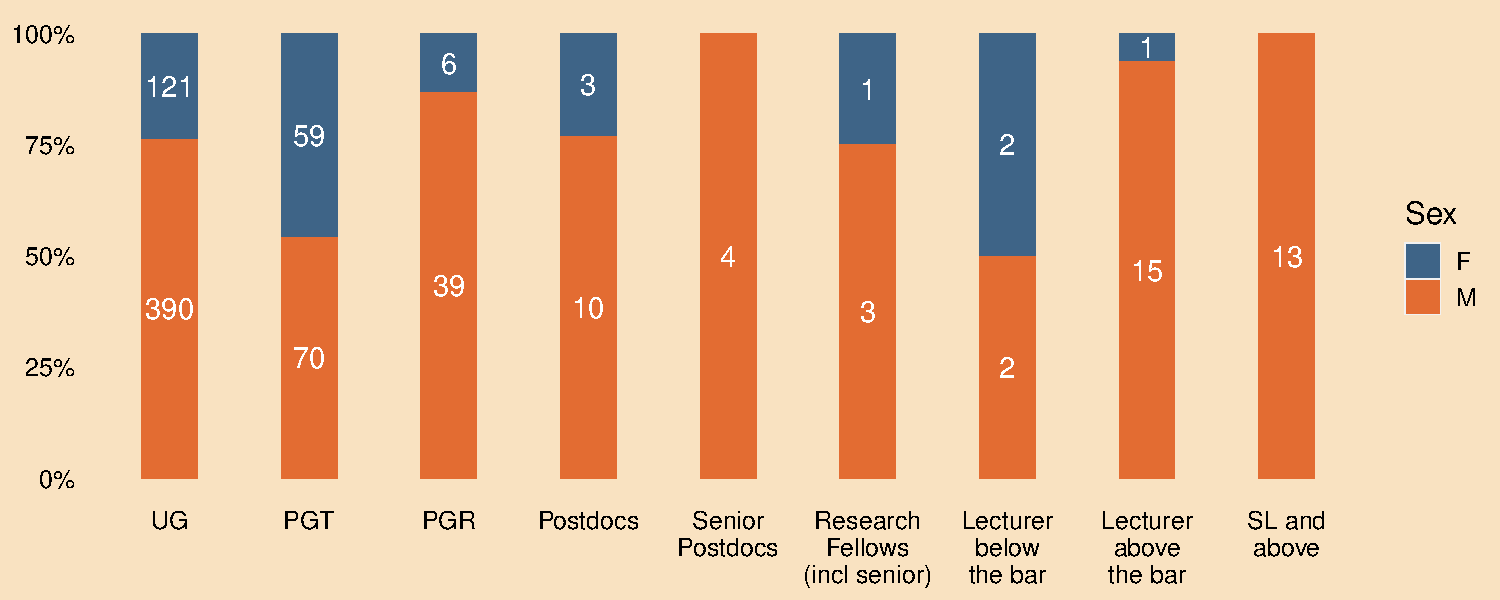
\includegraphics[width=5in]{fig/pipeline.pdf}
\end{figbox}

% \todo{[KJS: Insert figure "The career pipeline"; Tweak to include 
% undergraduates (24\%) and taught postgraduate (46\%) bars.
% See email of 2 Aug 2022.]}

The ``pipeline'' metaphor can result in an over-focus
on flow from beginning to end, potentially downplaying important 
inward flows at various stages. For example, very few Irish 
undergraduates progress to masters programmes, the healthly numbers
and gender balance in our PGT programmes is largely due to non-EU 
students entering the pipeline at masters level. Similarly, few  
masters graduates progress to PhD studies and PhD numbers are 
bolstered significantly by non-EU applicants. These inward flows
are welcome but do camouflage the dearth of female 
undergraduates to progress through PhD and onward to research and
academic careers.


The tapering proportion of females from undergraduates to lecturers to 
senior academics is a global phenomenon in computer science, but the 
complete lack of females in senior grades at UCC is an outlier even 
within our traditionally male-dominated discipline. 

The greatest choke points appear to be:
\begin{enumerate}[noitemsep]
    \item From undergraduate to PhD students
    \item From research roles to academic ones
    \item From lecturer to senior lecturer and beyond
\end{enumerate}

Relatively few CSIT graduates proceed to postgraduate studies 
(either taught masters or PhD) and many of our postgraduate 
students are  recruited from overseas, in particular China 
and India.
Employment prospects for Irish computing graduates are buoyant and, 
unlike other STEM disciplines, further postgraduate study is not a 
prerequisite for flourishing careers in  industry. Indeed, some of our 
undergraduates with expertise in sought-after fields such as computer 
security can be tempted by the prospect of lucrative 
job offers to leave even before their (undergraduate)
graduation.

The factors deterring research students and postdocs from pursuing 
academic careers are explored further in 
Section~\ref{sec:academic}. 
Poor PhD stipends (currently at \texteuro{}18,500 p.a.) and low
pay for postdoctoral positions relative to attractive industry salaries 
is one factor: starting salaries on offer to talented 
graduates can be a multiple of the PhD stipend. 
Precarity and the uncertainties surrounding  securing academic 
positions and promotional opportunities thereafter is another. 


As noted above, CSIT has no female academics at \ac{SL}
rank or above, so the Lecturer/SL boundary represents
a significant choke point.
At UCC academics can attain a senior grade 
either through promotion or direct appointment to an advertised 
position. Promotion criteria and processes at UCC are 
dictated entirely 
by the University and the School has had very limited success with 
promotions over the years.
In the past twenty years there have been six academic
promotions in all (none since 2014 and no females as CSIT did not have any female academics until 2017), 
but only three from Lecturer to 
SL (most recently in 2008).
In the most recent round (2018-2019), only two 
Lecturers from CSIT applied for promotion to SL, and neither was successful.  
If promotions are to contribute to improving gender balance at senior 
levels, the school will need to analyse historical barriers to promotion
and plan to more  proactively support colleagues, particularly
females, in navigating UCC's promotion scheme successfully. 

Section~\ref{sec:academic} explores staff experiences
and perception with recruitment and  promotions and presents a suite 
of actions to help improve the gender balance over 
time.


\subsection{Provide data for professional, managerial and support staff by gender and grade. Analyse representation, benchmarking where possible.}


% \khcomment{TCD website may allow benchmarking for sysadmin staff}

Table~\ref{tab:pmsstaff} gives an overview of the numbers of professional,
managerial and support staff. For historical reasons, UCC classifies
IT staff in the school's \ac{CSSS} as 
``administrative'' rather than ``technical.''

\input{tables2/tab_pms_staff}

Among those in administrative roles in the school's office, 
females predominate, while the School's core IT support staff 
are exclusively male. A similar pattern emerges among the 
administrative and IT roles among the research support staff.
This over-representation of females in administrative roles mirrors
the situation within the University.
Section~\ref{sec:pms} explores this issue in greater depth 
and presents actions to move the school on a more gender-balanced
trajectory for PMS staff.

By way of comparison, TCD's webpage currently lists 24 administrative 
staff (21 female, 3 male), nine IT support staff (three female, six
male) and six staff classified as technicians (all male).

\subsection{Provide data on staff on fixed-term contracts, contracts of indefinite duration/permanent contracts, and hourly-paid contracts by gender and staff category. Outline instances where fixed-term and hourly-paid contract types are used. This should include comment on:}
\instr{
\begin{itemize}
    \item whether or not numbers of fixed-term/hourly-paid contracts are representative of a typical year; 
    \item the rationale for the use of short-term contracts;
    \item the extent to which hourly-paid staff contribute to the teaching of core modules and/or services.
\end{itemize}
}

Table~\ref{tab:fthpstaff} summarises CSIT staff by category, contract 
type and gender for 2020.

\begin{tabbox}{!th}


\caption{CSIT staff by category, contract type and gender
(2020)}
\label{tab:fthpstaff}
\footnotesize 

      
\begin{tabular}{p{4cm}
                C{1cm}
                C{1cm}
                C{1cm}
                p{0.7cm}
                C{1cm}
                C{1cm}
                C{1cm}
                p{0.7cm}
                C{1cm}
                C{1cm}
                C{1cm}}
\toprule 
%\multicolumn{7}{c}{\bfseries Academics and Researchers (2020)}\\ \hline
  & \multicolumn{3}{c}{Permanent/CID} && \multicolumn{3}{c}{Fixed-Term} && \multicolumn{3}{c}{Hourly-Paid}\\
  \cmidrule{2-4}\cmidrule{6-8}\cmidrule{10-12}
  Category  & {F} & {M} & \%F && {F} & {M} & \%F && {F} & {M} & \%F\\
  \midrule 

  Academic&2 &27 &7\% &&1 & 3 & 25\% && - &1 & 0\%\\
  \hdashline 
  Researchers&- &- &- &&4 & 19 & 17\% && - &- &-\\
  \hdashline 
  PMS &8 &9  & 47\% & & 1 & - & - & & - & - &-\\
\bottomrule 
\end{tabular}

\end{tabbox}


\subsubsection{Representativeness of fixed-term/hourly paid contracts}

The broad pattern seen in the 2020 profile is fairly typical
of recent years. Hourly-paid contracts are never used for research 
or PMS roles and only rarely for academics, as noted below.


\subsubsection{Rationale for using short-term contracts}
\label{rationalecontracts}

Short term academic contracts (typically one year) are used 
to cover temporary vacancies in permanent posts arising from
maternity cover, retirements, etc. until the post can be filled on
a permanent basis. Also posts tied to new programmes are often
sanctioned on a fixed-term basis initially, but the School
actively advocates for these to be converted into permanent
posts.
% DT: Fixed terms 2020: LAB={RM}; LBB = {LM. JQ}
For example, two of the fixed-term lecturers shown in 
Table~\ref{tab:fthpstaff} have subsequently received 
permanent positions (both female).


Research activity is wholly dependent on the flow of research 
funding which is necessarily impermanent and so all researchers 
are on fixed-term contracts. A number of those in research 
administration or research IT support roles have core
permanent/\ac{CID} positions but who are appointed to a 
higher-grade role funded by research funds.

\subsubsection{Contribution of hourly-paid staff to teaching and services}

The bulk of hourly paid staff are undergraduate or postgraduate students
employed on a part-time basis as laboratory demonstrators or tutors for
undergraduate modules. The amount of such work varies from year to year 
but 2019-20, for example, we had 65 hourly paid staff, 11 female and 54 
male, i.e., about 17\% female, which is somewhat below the percentage of 
female  undergraduate and taught postgraduate  students.

A handful of modules (typically one to three modules per year out of 
around 100 in all) are covered by hourly-paid part-time lecturers,
generally postdocs seeking some teaching experience. Such arrangements
are used as sparingly as possible (three, two and one for 2017-18, 
2018-19, 2019-20 respectively) to cover gaps that would not justify 
or would be difficult to fill using a fixed-term contract.


% Dummy newcommand to mask errors due to old deleted actions.
\newcommand{\actdeptsurvey}{Deleted}
\newcommand{\actdeptmarketing}{Amended}
\newcommand{\actdeptrolemodels}{Amended}
\newcommand{\actdeptfunds}{Deleted}
\newcommand{\actdeptcareerchoice}{Amended}
\newcommand{\actdeptpromisingfemale}{Amended}
\newcommand{\actdeptringfence}{Deleted}
\newcommand{\actdepthighlight}{Amended}
\newcommand{\actdeptseminar}{Deleted}
\newcommand{\actdeptinternships}{Amended}



